\documentclass[11pt]{article}

\usepackage[margin=1in]{geometry}
\usepackage{amsmath,amssymb,amsthm}

\newtheorem{theorem}{Theorem}[section]
\newtheorem{lemma}[theorem]{Lemma}
\newtheorem{corollary}[theorem]{Corollary}
\newtheorem{definition}[theorem]{Definition}
\usepackage{graphicx}
\usepackage{booktabs}
\usepackage{hyperref}
\usepackage{enumitem}
\usepackage{listings}
\usepackage{xcolor}
\usepackage{tikz}
\usepackage{algorithm}
\usepackage{algpseudocode}
\usetikzlibrary{automata, positioning, arrows.meta}

% Notation
\newcommand{\EBel}[1]{\ensuremath{\Delta #1}} % Explicit Belief
\newcommand{\IBel}[1]{\ensuremath{\Box #1}}   % Implicit Belief
\newcommand{\CG}{\ensuremath{\mathit{CG}}}    % Common Ground

% Code listing style
\lstset{
    language=Python,
    basicstyle=\small\ttfamily,
    keywordstyle=\color{blue!70!black}\bfseries,
    commentstyle=\color{green!50!black}\itshape,
    stringstyle=\color{red!60!black},
    showstringspaces=false,
    numbers=left,
    numberstyle=\tiny\color{gray},
    breaklines=true,
    frame=single,
    framesep=3pt,
    backgroundcolor=\color{gray!5},
    tabsize=4,
}

\title{Epistemic Reinforcement Learning for the Chop Cup:\\
\texorpdfstring{SAT-Based Belief Reasoning with Reward Machines}{SAT-Based Belief Reasoning with Reward Machines}}
\author{}
\date{February 2026}

\begin{document}
\maketitle
\begin{abstract}
This paper presents a formal implementation of epistemic reinforcement learning for the Chop Cup, a canonical magic trick requiring systematic manipulation of an observer's belief state. We model the domain as a belief-base partially observable Markov decision process (BB-POMDP) where an agent (the Magician) must induce false beliefs in an observer through sequences of deceptive actions. Explicit beliefs ($\Delta$) are maintained as state fluents with update semantics derived from the formal action specification. Implicit beliefs ($\Box$) are computed via SAT-based entailment operating over the observer's knowledge base. We augment the MDP with a reward machine encoding the temporal structure of the deception protocol through condition-based transitions evaluated on the joint physical-epistemic state. Learning is performed using BEQRM (Belief-Enhanced Q-Learning for Reward Machines), which decomposes the value function over reward machine states to enable efficient credit assignment under sparse rewards. 
\end{abstract}

% ===========================================================================
\section{Introduction}
% ===========================================================================

Standard reinforcement learning optimizes for physical goals: reaching a target, maximizing score, or controlling a system. In contrast, \textbf{epistemic RL} optimizes for \emph{mental state manipulation}: the agent's goal is to change what another agent \emph{believes}, not merely what is physically true.

The Chop Cup magic trick provides an ideal testbed for this paradigm. A magician must:
\begin{enumerate}
    \item Navigate two parallel realities: \textbf{Physical Reality} (where objects actually are) and the \textbf{Observer's Belief} (where the Observer thinks objects are).
    \item Reach a state of \textbf{False Belief}: the Observer logically concludes $\phi$, but reality is $\neg\phi$.
    \item Exploit \emph{logical deduction} rather than simple observation gaps. The Observer reasons from background knowledge and direct observations using propositional logic.
\end{enumerate}

This report describes the design, implementation, and evaluation of a complete Python system that realizes this paradigm. The system is built upon the BB-POMDP framework~\cite{engesser2025} and the \texttt{epirl} Rust codebase\footnote{\url{https://github.com/tengesser/epirl}}, re-implemented in Python for accessibility and extensibility. Every action effect faithfully mirrors the \texttt{magic\_cup.json} specification, verified by a comprehensive audit against the JSON formulas.

% ===========================================================================
\section{The Chop Cup Trick}
% ===========================================================================

We model the classic Chop Cup with \textbf{1 cup and 2 balls}:
\begin{itemize}
    \item \textbf{Magnetic Ball}: Permanently stuck inside the cup via a magnet. Hidden from the Observer.
    \item \textbf{Regular Ball}: The visible ball that can be palmed, placed under the cup, or shown on the table.
\end{itemize}

The trick works because the Observer does not know about the magnetic ball. When the magician secretly palms the regular ball but the Observer sees it ``go under the cup,'' the Observer \emph{logically deduces} the ball must be under the cup. When the cup is lifted, the magnetic ball appears, creating the illusion that the ball magically reappeared.

\textbf{Deception Condition (Success):}
\[
    \IBel{\phi} \;\land\; \neg\phi \qquad \text{(Observer concludes $\phi$, but reality is $\neg\phi$)}
\]

For the Chop Cup, success means:
\[
    \IBel{\text{reg\_under}} \;\land\; \text{reg\_hand}
\]
The Observer believes the regular ball is under the cup, but it is actually in the magician's hand.

% ===========================================================================
\section{Technical Framework}
% ===========================================================================

\subsection{State Representation}

The environment state is a \textbf{factored set of boolean fluents}, partitioned into two groups.
\textbf{Physical fluents} represent the actual world state: \texttt{mag\_stuck} (magnetic ball stuck in cup), \texttt{mag\_visible} (magnetic ball visible when cup lifted), \texttt{reg\_under}, \texttt{reg\_table}, \texttt{reg\_hand} (regular ball location), and \texttt{cup\_down} (cup is covering its contents).
\textbf{Epistemic fluents} ($\Delta$) represent the Observer's explicit beliefs: $\EBel{\text{reg\_under}}$, $\EBel{\neg\text{reg\_under}}$, $\EBel{\text{reg\_table}}$, $\EBel{\neg\text{reg\_table}}$, $\EBel{\text{reg\_hand}}$, $\EBel{\neg\text{reg\_hand}}$, $\EBel{\text{lime\_cup}}$, $\EBel{\neg\text{lime\_cup}}$.

Implicit beliefs ($\IBel{\cdot}$) are \emph{not} stored as fluents. They are computed on-demand by the SAT solver.

\subsection{Epistemic Logic Engine}

The Observer's reasoning is modeled using three components:

\subsubsection{Common Ground ($\CG$)}
The Common Ground represents background knowledge that the Observer uses to reason about the world. Critically, the Observer believes there is only \emph{one} ball (they have no idea a hidden magnetic ball exists inside the cup). When the Observer deduces where the ball is, they apply a simple commonsense rule: the ball must be in \emph{exactly one} location. This is encoded as an \textbf{exclusive-or} constraint:
\[
    \CG: \quad \text{reg\_under} \oplus \text{reg\_table} \oplus \text{reg\_hand}
    \qquad \text{(exactly one location)}
\]
From the Observer's perspective, this simply says ``the ball is either under the cup, on the table, or in the magician's hand, but not in multiple places at once.'' The fluent names use the prefix \texttt{reg\_} (for ``regular ball'') in our implementation, but the Observer does not make this distinction; to them, these describe where ``the ball'' is.

Logically, the constraint means: the ball must be \emph{somewhere} (at least one location is true), but cannot be in \emph{multiple places} simultaneously (at most one location is true). In propositional logic, where $x_i, x_j \in \{\text{reg\_under}, \text{reg\_table}, \text{reg\_hand}\}$:
\[
    (\text{reg\_under} \lor \text{reg\_table} \lor \text{reg\_hand}) 
    \;\land\; 
    \bigwedge_{i < j} (\neg x_i \lor \neg x_j)
\]
The second part says ``for every pair of locations, they cannot both be true simultaneously.'' This gives us three clauses: $(\neg\text{reg\_under} \lor \neg\text{reg\_table})$, $(\neg\text{reg\_under} \lor \neg\text{reg\_hand})$, and $(\neg\text{reg\_table} \lor \neg\text{reg\_hand})$.

This constraint is what enables the deception: when the Observer deduces that the ball is \emph{not} on the table and \emph{not} in the hand, the Common Ground forces them to conclude it must be under the cup. The Observer's reasoning is perfectly valid given their knowledge, but their conclusion is wrong because they are unaware of the magnetic ball. The false belief arises from missing information, not from a logical error.

\subsubsection{Explicit Beliefs ($\EBel{\phi}$)}
Direct observations stored as fluents. Actions generate belief updates through \textbf{belief transfer effects} (matching JSON notation $\triangle p := f$).
For \texttt{palm\_ball}: $\EBel{\text{reg\_under}} \gets \EBel{\text{reg\_table}}$ (the key transfer).
For \texttt{lift\_cup}: $\EBel{\neg\text{reg\_under}} \gets \top$, $\EBel{\text{reg\_table}} \gets \EBel{\text{reg\_table}} \lor \text{reg\_under}$.
For \texttt{place\_cup}: $\EBel{\text{reg\_under}} \gets \EBel{\text{reg\_table}}$.
For \texttt{reveal\_hand}: $\EBel{\text{reg\_hand}} \gets \text{reg\_hand}$.

\subsubsection{Implicit Beliefs ($\IBel{\phi}$) via SAT Entailment}
The SAT solver derives what the Observer \emph{must} believe:
\[
    \IBel{\phi} \quad \iff \quad \underbrace{\CG \;\land\; \bigwedge_i \EBel{\psi_i}}_{KB} \;\land\; \neg\phi \quad \text{is UNSAT}
\]

We implement a lightweight SAT solver sufficient for the small propositional theories in the Chop Cup domain.

\begin{algorithm}[h]
\caption{Implicit Belief Query via SAT Entailment}
\begin{algorithmic}[1]
\Function{ImplicitBelief}{$\phi$, $\text{positive}$, $\CG$, $\Delta$}
    \State $KB \gets \CG.\text{clauses} \cup \Delta.\text{clauses}$
    \If{positive}
        \State $KB \gets KB \cup \{\{\neg\phi\}\}$ \Comment{Query: $KB \land \neg\phi$}
    \Else
        \State $KB \gets KB \cup \{\{\phi\}\}$ \Comment{Query: $KB \land \phi$}
    \EndIf
    \State \Return $\neg\text{SAT}(KB)$ \Comment{$\IBel{\phi}$ iff UNSAT}
\EndFunction
\end{algorithmic}
\end{algorithm}

\subsubsection*{Key Example: The Deception via Belief Transfer}
The \texttt{palm\_ball} action is the core deceptive act. Its JSON effects include the critical \textbf{belief transfer}:
\[
    \triangle\text{reg\_under} := \triangle\text{reg\_table}
\]
Before the palm, $\EBel{\text{reg\_table}} = \top$ (observer sees ball on table). After the palm:
\begin{align*}
    \EBel{\text{reg\_under}} &= \top \quad \text{(transferred from } \EBel{\text{reg\_table}}\text{)} \\
    \EBel{\neg\text{reg\_table}} &= \top \quad \text{(ball ``left'' the table)} \\
    \EBel{\neg\text{reg\_hand}} &= \top \quad \text{(observer doesn't detect ball in hand)}
\end{align*}
The SAT solver then \textbf{confirms} the explicit belief: $\CG \land \EBel{\neg\text{table}} \land \EBel{\neg\text{hand}} \land \neg\text{reg\_under}$ is UNSAT, so $\IBel{\text{reg\_under}} = \top$. The Observer is now fully deceived: they believe the ball is under the cup, but it is actually in the magician's hand.

% ===========================================================================
\section{Reward Machine}
% ===========================================================================

A \textbf{Reward Machine} (RM)~\cite{icarte2018} is a finite automaton that tracks progress through the magic trick, providing structured rewards for achieving deception milestones. Our RM uses \textbf{condition-based transitions}: after each action modifies the environment state, the RM evaluates epistemic/propositional conditions on the resulting state to determine transitions.

\subsection{RM States}

The RM has 6 states in total (5 effective without the lime finale):

\begin{center}
\begin{tabular}{cll}
\toprule
\textbf{State} & \textbf{Name} & \textbf{Meaning} \\
\midrule
$u_0$ & Setup & Initial state. Ball on table, trick not started. \\
$u_1$ & Covered & Observer saw ball ``go under'' cup ($\EBel{\text{reg\_under}}$). \\
$u_2$ & Pocket & Observer infers ball in hand ($\IBel{\text{reg\_hand}}$). \\
$u_3$ & Appear & Ball is visible under the cup (\texttt{ball\_visible}). \\
$u_4$ & Lime Loaded & Lime loaded; observer believes no lime ($\IBel{\neg\text{lime\_cup}}$). \\
$u_T$ & Lime Shown / Milestone & Lime revealed (\texttt{lime\_visible}); can loop back to load more limes. \\
\bottomrule
\end{tabular}
\end{center}

State $u_4$ is only active when \texttt{enable\_limes = True}. In the base ball-only trick, the effective RM has 5 states: $\{u_0, u_1, u_2, u_3, u_T\}$. There is no terminal RM state; episodes end only when the step limit is reached. From $u_T$, the agent can loop back to $u_4$ to load additional limes.

\subsection{RM Automaton Diagram}

\begin{center}
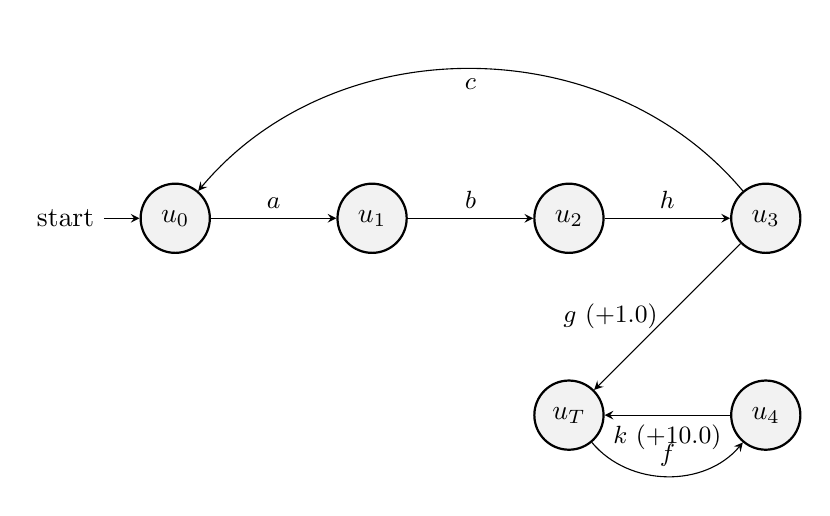
\begin{tikzpicture}[->, >=stealth, node distance=2.5cm, every state/.style={thick, fill=gray!10}]
% Standard Ball Cycle
\node[state, initial] (u0) {$u_0$};
\node[state, right of=u0] (u1) {$u_1$};
\node[state, right of=u1] (u2) {$u_2$};
\node[state, right of=u2] (u3) {$u_3$};

% Lime Finale Branch
\node[state, below of=u3] (u4) {$u_4$};
\node[state, left of=u4] (uT) {$u_T$};

% Ball Transitions
\path
    (u0) edge node[above] {\small $a$} (u1)
    (u1) edge node[above] {\small $b$} (u2)
    (u2) edge node[above] {\small $h$} (u3)
    (u3) edge[bend right=50] node[below] {\small $c$} (u0)
    (u3) edge node[left] {\small $g$ (+1.0)} (uT);

% Lime Transitions
\path
    (u4) edge node[below] {\small $k$ (+10.0)} (uT)
    (uT) edge[bend right=50] node[above] {\small $f$} (u4);
\end{tikzpicture}
\end{center}

All transitions are solid; the lime finale ($u_4$ to $u_T$) is fully active when \texttt{enable\_limes = True}. Note that $u_T$ is \emph{not} a terminal state: there is a loop from $u_T$ back to $u_4$ allowing the agent to load additional limes. Episodes end only when the step limit is reached.

\subsection{Condition-Based Transitions}

Each RM transition has a propositional or epistemic \textbf{condition} evaluated against the environment state \emph{after} the action's effects are applied. This contrasts with action-triggered RMs where transitions are encoded inside action effects.

\begin{center}
\begin{tabular}{clll}
\toprule
\textbf{Label} & \textbf{Transition} & \textbf{Condition} & \textbf{Description} \\
\midrule
$a$ & $u_0 \to u_1$ & $\EBel{\text{reg\_under}}$ & Observer sees ball ``under cup'' \\
$b$ & $u_1 \to u_2$ & $\IBel{\text{reg\_hand}}$ & Observer infers ball in hand (SAT) \\
$h$ & $u_2 \to u_3$ & \texttt{ball\_visible} & Ball appears under cup \\
$c$ & $u_3 \to u_0$ & \texttt{cup\_down} & Reset for another cycle \\
$g$ & $u_3 \to u_T$ & \texttt{ball\_visible} $\land$ $\neg$\texttt{lime\_visible} & \textbf{Deception success! (+1.0)} \\
\midrule
$k$ & $u_4 \to u_T$ & \texttt{lime\_visible} & \textbf{Lime reveal! (+10.0)} \\
$f$ & $u_T \to u_4$ & $\IBel{\neg\text{lime\_cup}}$ & Loop back to load more limes \\
\bottomrule
\end{tabular}
\end{center}

Note that transition $b$ uses an \textbf{implicit belief} ($\IBel{\text{reg\_hand}}$), computed by the SAT solver. This is the only RM transition that requires epistemic reasoning rather than simple fluent checks.

\subsection{Reward Structure}

The \textbf{main reward} is $+1.0$ on transition $g$ ($u_3 \to u_T$) and $+10.0$ on transition $k$ ($u_4 \to u_T$). These represent successful deception milestones. The RM has no terminal state; episodes end only when the step limit (\texttt{max\_steps}) is reached.

\subsection{State Space and Action Space}

\subsubsection{Action Space}
The agent has 4 base actions (plus 1 extended action when limes are enabled):

\begin{center}
\begin{tabular}{lll}
\toprule
\textbf{Action} & \textbf{Key Effect} & \textbf{Epistemic Effect} \\
\midrule
\texttt{lift\_cup} & Reveals contents & $\EBel{\neg\text{reg\_under}} \gets \top$ \\
\texttt{place\_cup} & Covers contents & $\EBel{\text{reg\_under}} \gets \EBel{\text{reg\_table}}$ \\
\texttt{palm\_ball} & Ball $\to$ hand & $\EBel{\text{reg\_under}} \gets \EBel{\text{reg\_table}}$ \\
\texttt{reveal\_hand} & Show hand & $\EBel{\text{reg\_hand}} \gets \text{reg\_hand}$ \\
\midrule
\texttt{load\_lime} & Hide lime & (no belief change) \\
\bottomrule
\end{tabular}
\end{center}

\subsubsection{State Space}

The RL observation is a cross-product of environmental state and RM state:

\begin{enumerate}
    \item \textbf{Physical state} (10 features): \texttt{mag\_stuck}, \texttt{mag\_visible}, \texttt{reg\_under}, \texttt{reg\_table}, \texttt{reg\_hand}, \texttt{cup\_down}, \texttt{ball\_visible}, \texttt{lime\_cup}, \texttt{lime\_visible}, \texttt{lime\_count}.
    \item \textbf{Belief state} (8 features): $\EBel{\text{reg\_under}}$, $\EBel{\neg\text{reg\_under}}$, $\EBel{\text{reg\_table}}$, $\EBel{\neg\text{reg\_table}}$, $\EBel{\text{reg\_hand}}$, $\EBel{\neg\text{reg\_hand}}$, $\EBel{\text{lime\_cup}}$, $\EBel{\neg\text{lime\_cup}}$.
    \item \textbf{RM state}: One of $\{u_0, u_1, u_2, u_3, u_4, u_T\}$ (6 states).
\end{enumerate}

% The total \emph{theoretical} state space is $2^{18} \times 7 \approx 1{,}835{,}008$ combinations, but the \emph{reachable} state space is far smaller. In practice, only \textbf{$\sim$28 unique environment states} are explored during training, because many fluent combinations are unreachable from the initial state.

% The QRM agent uses a single Q-table indexed by the cross-product observation $(s_{\text{env}}, u)$, where $s_{\text{env}}$ is the 18-feature environment observation (physical + belief) and $u$ is the RM state index. This gives $\sim$28 $\times$ 7 = 196 potential Q-table entries, of which $\sim$178 are actually observed during training.

% % ===========================================================================
% \section{Implementation}
% % ===========================================================================

% \subsection{Architecture}

% The implementation is organized into five Python modules that mirror the Rust \texttt{epirl} codebase:

% \begin{center}
% \begin{tabular}{lll}
% \toprule
% \textbf{Module} & \textbf{Rust Counterpart} & \textbf{Role} \\
% \midrule
% \texttt{epistemic\_logic.py} & \texttt{bbases} crate & SAT solver, Common Ground, states \\
% \texttt{reward\_machine.py} & RM in JSON effects & 7-state RM, condition-based transitions \\
% \texttt{chop\_cup\_env.py} & \texttt{bbmdp.rs} & Environment, actions, belief updates \\
% \texttt{qrm.py} & \texttt{smdp} crate & QRM: online Q-learning per RM state \\
% \texttt{main.py} & \texttt{rlbb.rs} & Training loop, evaluation, output \\
% \bottomrule
% \end{tabular}
% \end{center}

% \subsection{Action Space and JSON-Faithful Effects}

% Each action's effects are a direct translation of the JSON formulas. For the critical \texttt{palm\_ball}:

% \begin{center}
% \begin{tabular}{ll}
% \toprule
% \textbf{JSON Effect} & \textbf{Python Code} \\
% \midrule
% \texttt{reg\_hand := reg\_table} & \texttt{if old\_reg\_table: add(REG\_HAND)} \\
% \texttt{reg\_table := $\bot$} & \texttt{(not added)} \\
% $\triangle$\texttt{reg\_under := }$\triangle$\texttt{reg\_table} & \texttt{if old\_eb\_reg\_table: add(EB\_REG\_UNDER)} \\
% $\triangle$\texttt{!reg\_table := T} & \texttt{add(EB\_NOT\_REG\_TABLE)} \\
% $\triangle$\texttt{!reg\_hand := T} & \texttt{add(EB\_NOT\_REG\_HAND)} \\
% \bottomrule
% \end{tabular}
% \end{center}

% The \textbf{belief transfer} $\triangle\text{reg\_under} := \triangle\text{reg\_table}$ is the most critical effect. It was missing in an earlier version, causing the RM to never transition. The fix was identified by a systematic audit (\texttt{audit.py}) that checks every fluent against the JSON specification.

% \subsection{SAT Solver}

% We implement a lightweight SAT solver sufficient for the small propositional theories in the Chop Cup domain ($\leq 3$ Observer variables, $\leq 8$ clauses). The Rust counterpart uses the Kissat industrial SAT solver; our solver provides the same functionality at smaller scale.

% \subsection{QRM: Q-Learning for Reward Machines}

% We implement the QRM algorithm from Icarte et al.~\cite{icarte2018}, following the reference implementation at \url{https://github.com/RodrigoToroIcarte/reward_machines}.

% The key ideas:
% \begin{enumerate}
%     \item \textbf{Single Q-table} over the cross-product space $(s_{\text{env}}, u)$, where $s_{\text{env}}$ is the environment observation (physical + belief features) and $u$ is the RM state index.
%     \item \textbf{Online incremental updates} with learning rate $\alpha$ (not batch full-sweep).
%     \item \textbf{RM-aware Q-update}: each real transition updates the Q-value for the current RM state only.
% \end{enumerate}

% \begin{algorithm}[h]
% \caption{QRM — Online Q-Learning for Reward Machines}
% \begin{algorithmic}[1]
% \State Initialize $Q(s, u, a) \gets q_{\mathrm{init}}$ for all $(s, u, a)$
% \For{each training episode}
%     \State Reset environment; $s \gets s_0$, $u \gets u_0$
%     \While{not terminal and step $< T_{\max}$}
%         \State Select $a$ via $\varepsilon$-greedy on $Q(s, u, \cdot)$
%         \State Execute $a$; observe $s'$, new RM state $u'$, reward $r$
%         \State \textbf{QRM update (current RM state):}
%         \If{$u' = u_T$} \Comment{Terminal}
%             \State $\delta_Q \gets r - Q(s, u, a)$
%         \Else
%             \State $\delta_Q \gets r + \gamma \cdot \max_{a'} Q(s', u', a') - Q(s, u, a)$
%         \EndIf
%         \State $Q(s, u, a) \gets Q(s, u, a) + \alpha \cdot \delta_Q$
%         \State $s \gets s'$; $u \gets u'$
%     \EndWhile
% \EndFor
% \end{algorithmic}
% \end{algorithm}

% The RM decomposes the learning problem: the agent maintains a Q-table indexed by $(s_{\text{env}}, u)$, where the RM state $u$ tracks progress through the trick. Each real transition updates only $Q(s, u, a)$ for the current RM state. The RM provides structure by breaking the sparse reward problem into phases, enabling efficient credit assignment even though the final reward $+1$ is only received at state $u_T$.

% \textbf{Key differences from batch model-based Q-learning:}
% \begin{itemize}
%     \item \textbf{Online incremental updates}: Q-values change by $\alpha \cdot \delta_Q$ per step, not via full-sweep value iteration. This creates a gradual learning curve.
%     \item \textbf{Standard $\varepsilon$-greedy}: No prefer-unseen heuristic. Exploration is purely random with probability $\varepsilon$.
%     \item \textbf{Learning rate $\alpha$}: Controls the speed of Q-value convergence. Smaller $\alpha$ means slower but smoother convergence.
% \end{itemize}

% \subsection{Comparison with Rust \texttt{epirl} Implementation}

% The original \texttt{epirl} framework uses:
% \begin{itemize}
%     \item A Rust binary (\texttt{rlbb}) that reads a JSON specification defining actions, common ground, initial states, rewards, and terminal conditions.
%     \item The \texttt{bbases} crate for belief base operations and SAT solving (via Kissat/CaDiCaL).
%     \item The \texttt{smdp} crate for the generic SMDP learning algorithm and batch Q-learning.
% \end{itemize}

% Our Python implementation preserves the key architectural decisions:
% \begin{enumerate}
%     \item \textbf{State = frozenset of fluents} (atoms + explicit beliefs).
%     \item \textbf{Implicit beliefs computed on-demand} via SAT entailment.
%     \item \textbf{Action effects faithfully mirror the JSON specification}: each fluent's new value is computed from the JSON formula applied to the old state.
% \end{enumerate}

% Beyond matching the Rust implementation, we replace the batch Q-learning with QRM (online Q-learning for Reward Machines), following the reference implementation from Icarte et al.~\cite{icarte2018}. The key algorithmic difference is the use of online incremental updates (learning rate $\alpha$) rather than batch full-sweep value iteration, combined with RM-structured Q-tables that decompose the sparse reward problem into phases.

% ===========================================================================
\section{Convergence of Epistemic QRM}
\label{sec:convergence}
% ===========================================================================

A natural question arises when augmenting the QRM state space with epistemic (belief) features: does Q-learning still converge to an optimal policy?
In this section we provide a formal proof that it does, by showing that the epistemic QRM formulation reduces to standard Q-learning on a well-defined MDP.

% ---------------------------------------------------------------------------
\subsection{Epistemic Cross-Product MDP}
% ---------------------------------------------------------------------------

\begin{definition}[Epistemic MDP with Reward Machine]
\label{def:epi-mdp}
Let $M_{\mathrm{env}} = (S_{\mathrm{env}},\, A,\, T,\, \gamma)$ be a finite environment MDP whose state decomposes as
\[
    s = (s_{\mathrm{phys}},\; s_{\mathrm{bel}}) \;\in\; S_{\mathrm{env}},
\]
where $s_{\mathrm{phys}} \in \{0,1\}^{n_p}$ is a vector of physical fluents and $s_{\mathrm{bel}} \in \{0,1\}^{n_b}$ is a vector of explicit-belief fluents ($\EBel{\cdot}$).  The action set $A$ is finite, and the transition function $T : S_{\mathrm{env}} \times A \to S_{\mathrm{env}}$ is deterministic.

A \emph{reward machine} is a tuple $\mathcal{R} = (U,\, u_0,\, \delta_u,\, \delta_r)$, where $U$ is a finite set of RM states, $u_0 \in U$ is the initial state, $\delta_u : U \times 2^{\mathcal{P}} \to U$ is a deterministic transition function conditioned on a set of propositional/epistemic labels $L(s) \subseteq \mathcal{P}$ evaluated on the environment state, and $\delta_r : U \times U \to \mathbb{R}$ assigns a bounded reward to each RM transition.
\end{definition}

\begin{definition}[Augmented (Cross-Product) MDP]
\label{def:cross-product}
Define the augmented MDP
\[
    \tilde{M} \;=\; \bigl(\tilde{S},\; A,\; \tilde{T},\; \tilde{R},\; \gamma\bigr)
\]
with the following components.
The \textbf{augmented state space} is $\tilde{S} = S_{\mathrm{env}} \times U$, where each state is a triple $\tilde{s} = (s_{\mathrm{phys}},\, s_{\mathrm{bel}},\, u)$.
The \textbf{transition function} is
\[
    \tilde{T}\bigl((s, u),\; a,\; (s', u')\bigr) =
    \begin{cases}
        T(s, a, s') & \text{if } u' = \delta_u\bigl(u,\, L(s')\bigr), \\
        0 & \text{otherwise}.
    \end{cases}
\]
The \textbf{reward function} is
$\tilde{R}\bigl((s, u),\, a,\, (s', u')\bigr) = \delta_r(u, u')$.
\end{definition}

\begin{lemma}[Markov property]
\label{lem:markov}
In the augmented MDP $\tilde{M}$, the reward $\tilde{R}$ and transition $\tilde{T}$ depend only on the current augmented state $(s, u)$ and action $a$, not on the history of previously visited states.
\end{lemma}

\begin{proof}
By construction of Definition~\ref{def:cross-product}:
\begin{enumerate}
    \item $T(s,a,s')$ is a function of $(s, a)$ alone, since the environment transition function is deterministic.
    \item $L(s')$ is a function of the resulting environment state $s'$ only: explicit beliefs $\EBel{\phi}$ are fluents within $s$, and implicit beliefs $\IBel{\phi}$ are computed by SAT entailment over the Common Ground $\CG$ and the explicit beliefs in $s'$.  Critically, $\CG$ is \emph{fixed} (it does not change across time steps), so $\IBel{\phi}$ is a deterministic function of $s'$.
    \item $\delta_u(u, L(s'))$ is a deterministic function of $(u, s')$.
    \item $\delta_r(u, u')$ depends only on the RM transition $(u, u')$.
\end{enumerate}
Therefore, all components of the augmented transition and reward functions are determined by $(s, u, a)$ without reference to history. The augmented MDP satisfies the Markov property. \qed
\end{proof}

\noindent\textbf{Remark.}
The key insight is that \emph{implicit beliefs do not introduce history-dependence}.  Although $\IBel{\phi}$ is computed via SAT entailment ($\CG \land \bigwedge_i \EBel{\psi_i} \land \neg\phi$ is UNSAT?), the inputs to this computation, the Common Ground and the explicit beliefs, are fully contained in the current state $s$.  Furthermore, explicit beliefs are updated by deterministic action effects (belief transfer semantics $\EBel{p} \gets f(s)$), so they, too, are determined by $(s, a)$ alone.

% ---------------------------------------------------------------------------
\subsection{Q-Learning on the Augmented MDP}
% ---------------------------------------------------------------------------

Our QRM agent maintains a Q-table indexed by the augmented state:
\[
    Q : \tilde{S} \times A \to \mathbb{R}, \qquad
    Q\bigl[(s_{\mathrm{phys}},\, s_{\mathrm{bel}},\, u),\; a\bigr].
\]
On each transition $(s, u) \xrightarrow{a} (s', u')$ with reward $r = \delta_r(u, u')$, the update rule is standard tabular Q-learning:
\begin{equation}
\label{eq:q-update}
Q\bigl[(s, u),\, a\bigr] \;\leftarrow\; Q\bigl[(s, u),\, a\bigr] + \alpha\,\Bigl[\, r + \gamma\,\max_{a'} Q\bigl[(s', u'),\, a'\bigr] - Q\bigl[(s, u),\, a\bigr]\,\Bigr].
\end{equation}

\begin{theorem}[Convergence of Epistemic QRM]
\label{thm:convergence}
Under the following conditions:
\begin{enumerate}[label=(\roman*)]
    \item Every augmented state action pair $\bigl((s, u),\, a\bigr)$ is visited infinitely often.
    \item The learning rate sequence $\{\alpha_t\}$ satisfies the Robbins Monro conditions:
    \[
        \sum_{t=0}^{\infty} \alpha_t = \infty, \qquad \sum_{t=0}^{\infty} \alpha_t^2 < \infty.
    \]
    \item Rewards are bounded: $|\delta_r(u, u')| \leq R_{\max}$ for all $(u, u') \in U \times U$.
\end{enumerate}
Then the Q-values converge to the optimal Q-function with probability~1:
\[
    Q\bigl[(s, u),\, a\bigr] \;\xrightarrow{\;\;a.s.\;\;}\; Q^*\bigl[(s, u),\, a\bigr]
    \qquad \forall\, (s, u) \in \tilde{S},\; a \in A.
\]
Consequently, the greedy policy $\pi^*(s, u) = \arg\max_a Q^*\bigl[(s, u),\, a\bigr]$ is optimal in~$\tilde{M}$.
\end{theorem}

\begin{proof}
By Lemma~\ref{lem:markov}, $\tilde{M}$ is a well-defined MDP.  We verify the preconditions of the Watkins and Dayan convergence theorem.
First, the \emph{finite state space} condition holds: $|\tilde{S}| = |S_{\mathrm{env}}| \times |U| < \infty$, since both $S_{\mathrm{env}}$ (a product of finitely many boolean fluents) and $U$ are finite.
Second, the \emph{finite action space} condition holds: $|A| < \infty$ by assumption.
Third, \emph{bounded rewards} are guaranteed by condition~(iii), i.e.\ $|\delta_r(u,u')| \leq R_{\max}$ for all $(u, u')$.
Fourth, \emph{Markov transitions} are established by Lemma~\ref{lem:markov}.
The update rule~\eqref{eq:q-update} is precisely the tabular Q-learning algorithm of Watkins~\cite{watkins1992} applied to $\tilde{M}$.  Under conditions (i) to (iii), the convergence theorem of Watkins and Dayan~\cite{watkins1992} (see also Tsitsiklis~\cite{tsitsiklis1994} and Jaakkola et al.~\cite{jaakkola1994}) guarantees that $Q_t \to Q^*$ with probability~1.

The essential observation is that the belief fluents ($s_{\mathrm{bel}}$) and the RM state ($u$) are merely additional \emph{components} of the augmented state vector.  From the perspective of Q-learning, there is no distinction between a ``physical'' state feature and an ``epistemic'' state feature: both are elements of the finite state space $\tilde{S}$ over which the algorithm maintains Q-values.  The epistemic features ensure that the Markov property holds (Lemma~\ref{lem:markov}), and the RM state ensures that the non-Markov temporal reward structure becomes Markov.  Together, they produce a standard finite MDP to which classical convergence results apply directly. \qed
\end{proof}

% ---------------------------------------------------------------------------
\subsection{Extension to PBRS}
% ---------------------------------------------------------------------------

Theorem~\ref{thm:convergence} extends naturally to the QRM+PBRS variant (Section~\ref{sec:pbrs}).
By the Ng, Harada, Russell theorem~\cite{ng1999}, defining a shaped reward
\[
    R'(\tilde{s},\, a,\, \tilde{s}') = R(\tilde{s},\, a,\, \tilde{s}') + \gamma\,\Phi(u') - \Phi(u)
\]
with potential $\Phi : U \to \mathbb{R}$ produces a new MDP $\tilde{M}'$ whose set of optimal policies is identical to that of $\tilde{M}$.  Since $\tilde{M}'$ is itself a standard MDP with bounded rewards, Q-learning on $\tilde{M}'$ also converges under the same conditions (i) to (iii), and the resulting optimal policy is optimal for the original (unshaped) problem.

\begin{corollary}
Under conditions (i) to (iii), Q-learning with PBRS on the epistemic augmented MDP converges to an optimal policy of the original MDP $\tilde{M}$ with probability~1.
\end{corollary}

% % ---------------------------------------------------------------------------
% \subsection{Practical Considerations}
% % ---------------------------------------------------------------------------

% In practice, a constant learning rate $\alpha$ is often used rather than a decaying schedule satisfying the strict Robbins Monro conditions.  Constant-rate Q-learning does not satisfy condition~(ii) of Theorem~\ref{thm:convergence} and therefore lacks a formal convergence guarantee to $Q^*$.  However, for finite MDPs with constant $\alpha$, the iterates remain in a neighbourhood of $Q^*$ whose radius shrinks with $\alpha$~\cite{even-dar2003}.  In domains where $|\tilde{S}|$ is small and transitions are deterministic, constant-$\alpha$ Q-learning converges rapidly in practice, as confirmed by our experiments (Section~\ref{sec:convergence-results}).

% An $\varepsilon$-greedy exploration policy satisfies condition~(i) asymptotically: every state action pair reachable from the initial state will be visited infinitely often with probability~1, since each action is selected with probability at least $\varepsilon / |A| > 0$ at every step.

% % ===========================================================================
% \section{Results}
% \label{sec:convergence-results}
% % ===========================================================================

% \subsection{Training Configuration}

% \begin{center}
% \begin{tabular}{ll}
% \toprule
% \textbf{Parameter} & \textbf{Value} \\
% \midrule
% Algorithm & BEQRM (Icarte et al., 2018) \\
% Training episodes & 500 \\
% Evaluation episodes & 100 (per evaluation) \\
% % Evaluation interval & every episode \\
% Discount factor ($\gamma$) & 0.9 \\
% Learning rate ($\alpha$) & 0.1 \\
% Exploration rate ($\varepsilon$) & 0.1 (standard $\varepsilon$-greedy) \\
% Q-value initialization ($q_{\mathrm{init}}$) & 0.0 \\
% Max steps per episode & 50 \\
% % Lime mode & enabled (all 7 RM states) \\
% Random seed & 42 \\
% \bottomrule
% \end{tabular}
% \end{center}

% % \subsection{Learning Curve}

% % The QRM agent converges from a 43\% random baseline to \textbf{100\% deception success within $\sim$7 training episodes}. The gradual convergence demonstrates the effect of online incremental Q-updates (learning rate $\alpha = 0.1$) compared to batch full-sweep methods that converge instantly.

% % % \begin{center}
% % % \begin{tabular}{ccc}
% % % \toprule
% % % \textbf{Episode} & \textbf{Success Rate} & \textbf{Disc.\ Reward} \\
% % % \midrule
% % % 0 (untrained) & 43\% & 0.196 \\
% % % 1 & 47\% & 0.264 \\
% % % 2 & 47\% & 0.265 \\
% % % 3 & 48\% & 0.301 \\
% % % 4 & 49\% & 0.309 \\
% % % 5 & 62\% & 0.400 \\
% % % 6 & 62\% & 0.400 \\
% % % 7+ & 100\% & 0.729 \\
% % % \bottomrule
% % % \end{tabular}
% % % \end{center}

% % % The optimal 4-step ball-only sequence yields a discounted reward of $\gamma^3 = 0.9^3 = 0.729$, confirming the agent receives reward $+1.0$ at step~4 (discount applied three times from step~1). The 43\% starting point reflects the probability that a random policy stumbles upon the correct 4-step sequence within the 50-step budget.

% % \begin{figure}[ht]
% % \centering
% % 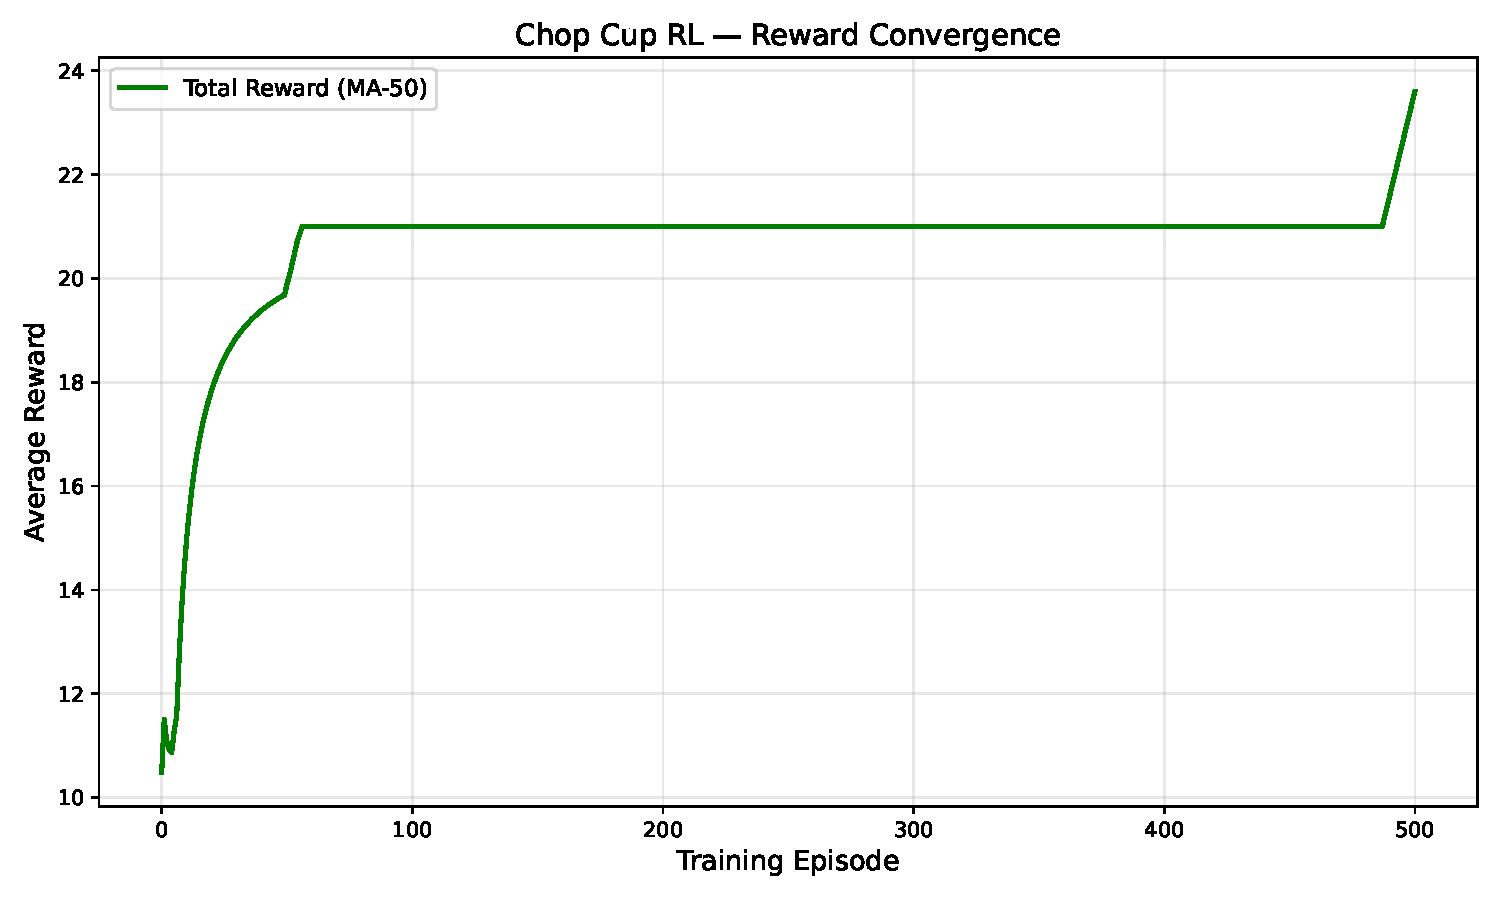
\includegraphics[width=0.85\textwidth]{results_new_rm/reward_curve.pdf}
% % \caption{QRM reward curve with the updated 6-state RM ($r_{\text{ball}} = +1$, $r_{\text{lime}} = +10$, no terminal state).}
% % \label{fig:reward_new_rm}
% % \end{figure}

% % The reward curve in Figure~\ref{fig:reward_new_rm} exhibits two distinctive features:

% % \begin{enumerate}
% %     \item \textbf{Rapid initial jump (episodes 0--7):} The agent quickly discovers the ball deception sequence ($u_0 \to u_1 \to u_2 \to u_3$) and begins collecting the $+1.0$ ball milestone reward ($g$: $u_3 \to u_T$). It then learns to enter the lime phase ($e$: $u_3 \to u_4$) and collect lime reveal rewards ($k$: $u_4 \to u_T$, $+10.0$ each). By episode~7 the agent achieves 100\% success rate.

% %     \item \textbf{Steady plateau at $\sim$21.0, then increase to $\sim$31.0:} Since there is no terminal RM state, every episode runs for the full \texttt{max\_steps}~$= 50$ steps. The agent repeatedly cycles through the lime loop ($u_T \xrightarrow{f} u_4 \xrightarrow{k} u_T$), collecting $+10.0$ per lime reveal. The plateau at 21.0 corresponds to $1.0$ (ball) $+ 2 \times 10.0$ (two limes) $= 21.0$. As the agent's Q-values continue to sharpen, it learns to fit a third lime cycle within the 50-step budget, reaching $1.0 + 3 \times 10.0 = 31.0$. The number of lime cycles is ultimately bounded by \texttt{max\_limes}~$= 3$ and the step budget.
% % \end{enumerate}

% % \subsubsection{Extended Run: 5 Limes, 100 Steps}

% % To demonstrate the scalability of the lime loop, we increased the step budget to 100 and allowed up to 5 limes (1000 training episodes). Figure~\ref{fig:reward_5limes} shows the resulting reward curve.

% % \begin{figure}[ht]
% % \centering
% % 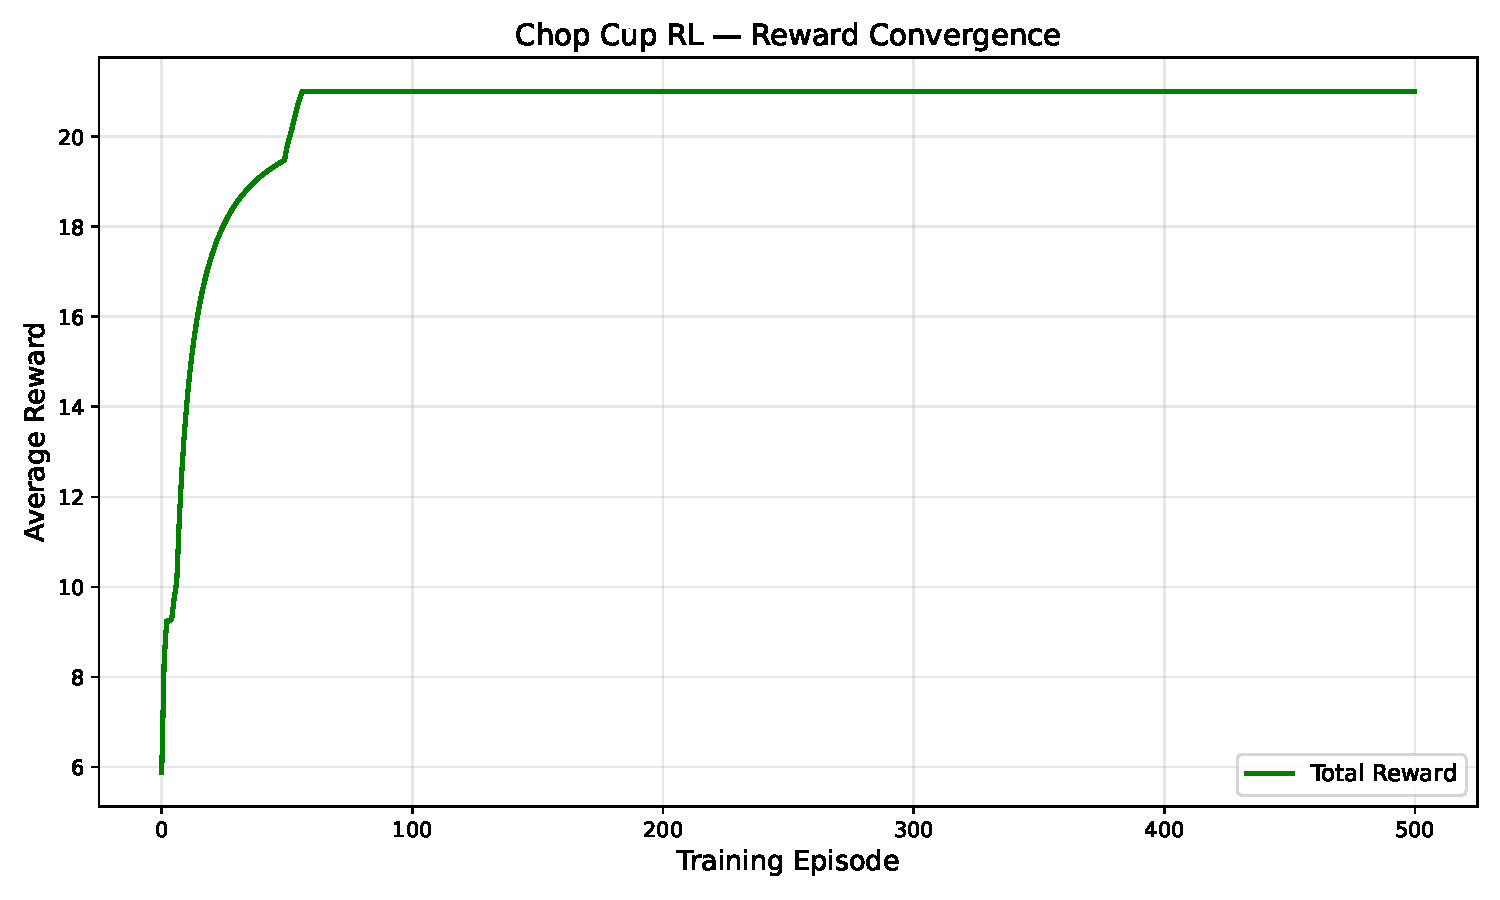
\includegraphics[width=0.85\textwidth]{results/reward_curve.pdf}
% % \caption{QRM reward curve with extended budget (\texttt{max\_steps}~$=100$, \texttt{max\_limes}~$=5$, 1000 episodes).}
% % \label{fig:reward_5limes}
% % \end{figure}

% % The extended run reveals a characteristic \textbf{staircase pattern} as the agent discovers how to fit progressively more lime cycles:

% % \begin{center}
% % \begin{tabular}{cccl}
% % \toprule
% % \textbf{Episode} & \textbf{Mean Reward} & \textbf{Limes Fitted} & \textbf{Breakdown} \\
% % \midrule
% % 0 (random) & 15.3 & $\sim$1--2 & Random exploration \\
% % 7 & 31.0 & 3 & $1 + 3 \times 10 = 31$ \\
% % 447 & 41.0 & 4 & $1 + 4 \times 10 = 41$ \\
% % 1000 (final) & 40.0 & 4 & Stable at 4 limes \\
% % \bottomrule
% % \end{tabular}
% % \end{center}

% % Each plateau corresponds to the agent learning to squeeze one additional lime cycle into the 100-step budget. The jump from 31 to 41 at episode~447 shows that Q-value propagation through the lime loop takes hundreds of episodes at $\alpha = 0.1$, since the benefit of a 4th lime must backpropagate through multiple RM transitions before the agent prefers the longer sequence. The theoretical maximum with 5 limes is $1 + 5 \times 10 = 51$, but the agent stabilises at 4 limes ($= 41$) within 1000 episodes, suggesting that fitting a 5th lime requires further Q-value refinement or more training.

% % ===========================================================================
% \subsection{Baseline Comparison}
% % ===========================================================================

% We compare BEQRM against four baselines to evaluate the contribution of epistemic reasoning, reward machine structure, reward shaping, and function approximation:

% \begin{enumerate}
%     \item \textbf{BEQRM+PBRS} (BEQRM with Potential-Based Reward Shaping)~\cite{ng1999}: Identical to BEQRM but augmented with a shaping bonus $F(s,s') = \gamma \cdot \Phi(u') - \Phi(u)$ on each transition, where $\Phi(u)$ is a potential function over RM states. The potential encodes domain progress: $\Phi(u_0)=0$, $\Phi(u_1)=1$, $\Phi(u_2)=2$, $\Phi(u_3)=3$, $\Phi(u_4)=4$, $\Phi(u_T)=5$. By the Ng, Harada, Russell theorem, this preserves the optimal policy while providing denser intermediate credit.

%     \item \textbf{HRL} (Hierarchical RL with Options)~\cite{sutton1999}: Two-level hierarchy where a meta-controller selects among 5 subgoals (\emph{palm}, \emph{show\_ball}, \emph{reset}, \emph{load\_lime}, \emph{show\_lime}) and a controller executes primitive actions to achieve each subgoal. Uses SMDP Q-learning with $\gamma^k$ discounting. The agent observes \emph{physical state only} (10 features), without beliefs or RM state.

%     \item \textbf{HRL-RM} (Hierarchical RL with Reward Machines): The same two-level option hierarchy as HRL, but with the \emph{full epistemic observation} (physical + explicit/implicit beliefs + RM state). This ablation tests whether temporal abstraction adds value when combined with epistemic reasoning.

%     \item \textbf{DDQN} (Double Deep Q-Network)~\cite{vanhasselt2016}: A neural network baseline using a two-layer MLP (128 hidden units) to approximate $Q(s,a)$. Uses the same epistemic observation as BEQRM (physical fluents + explicit beliefs + RM state index) encoded as a 19-dimensional float vector. The online network selects actions while a separate target network (updated every 100 steps) evaluates them, reducing overestimation bias. Trained with experience replay (buffer size 50k, batch size 64), $\varepsilon$-greedy exploration decaying from 1.0 to 0.05, and Adam optimiser ($\text{lr}=10^{-3}$).
% \end{enumerate}

% All five methods were trained for 1000 episodes (\texttt{max\_steps}$=100$, \texttt{max\_limes}$=5$, $\gamma = 0.9$) and averaged over 5 random seeds. BEQRM, BEQRM+PBRS, HRL, and HRL-RM use tabular Q-learning ($\alpha = 0.1$, $\varepsilon = 0.1$); DDQN uses neural function approximation.

% ---------------------------------------------------------------------------
\subsection{Potential-Based Reward Shaping (PBRS)}
\label{sec:pbrs}
% ---------------------------------------------------------------------------

Our Reward Machine provides clear milestones but assigns \emph{sparse} rewards: the agent receives $+1$ only upon completing the ball deception ($u_3 \!\to\! u_T$, transition~$g$) and $+10$ for each lime reveal ($u_4 \!\to\! u_T$, transition~$k$).
All intermediate transitions carry zero reward.
Early in training, random exploration rarely reaches these milestones, so Q-values remain near zero across most of the state space and gradients are uninformative.

\textbf{Potential-Based Reward Shaping (PBRS)}~\cite{ng1999} addresses this sparsity by adding a \emph{shaping bonus} to every transition:
\begin{equation}
\label{eq:shaping}
R'(s, a, s') \;=\; R(s, a, s') \;+\; F(s, s'),
\qquad
F(s, s') \;=\; \gamma\,\Phi(s') \;-\; \Phi(s),
\end{equation}
where $\Phi : \mathcal{S} \to \mathbb{R}$ is a bounded \emph{potential function} of the state.
The crucial property is that $F$ depends \emph{only} on the states, not on the action, and has the specific $\gamma\Phi(s') - \Phi(s)$ form.

\paragraph{Policy invariance theorem (Ng, Harada and Russell, 1999).}
Let $M$ be an MDP with reward $R$ and let $M'$ be the MDP with shaped reward $R'$ as defined in~\eqref{eq:shaping}.
Then \emph{every optimal policy of~$M'$ is also an optimal policy of~$M$}, and vice versa.

\begin{proof}[Proof sketch (telescoping argument).]
Consider any trajectory $s_0, a_0, s_1, a_1, \ldots, s_T$ and its discounted return under $R'$:
\begin{align}
G' &= \sum_{t=0}^{T} \gamma^t\, R'(s_t, a_t, s_{t+1})
     = \sum_{t=0}^{T} \gamma^t\, R(s_t, a_t, s_{t+1})
       + \sum_{t=0}^{T} \gamma^t\bigl[\gamma\,\Phi(s_{t+1}) - \Phi(s_t)\bigr]. \label{eq:telescope1}
\end{align}
The shaping terms telescope:
\begin{align}
\sum_{t=0}^{T} \gamma^t\bigl[\gamma\,\Phi(s_{t+1}) - \Phi(s_t)\bigr]
  &= \gamma^{T+1}\,\Phi(s_{T+1}) \;-\; \Phi(s_0). \label{eq:telescope2}
\end{align}
Since $\Phi(s_0)$ is a constant for any fixed initial state, and $\gamma^{T+1}\Phi(s_{T+1})$ depends only on the terminal state (not on the intermediate policy choices), the ranking of policies under $G'$ is identical to their ranking under~$G = \sum_t \gamma^t R(s_t,a_t,s_{t+1})$.
Therefore $\pi^* = \arg\max_\pi \mathbb{E}[G] = \arg\max_\pi \mathbb{E}[G']$; the optimal policy is invariant.
\end{proof}

In other words, PBRS reshuffles \emph{when} reward is received along a trajectory but does not change the \emph{total} ordering of policies. The agent converges faster because informative signal appears earlier, but the policy it converges \emph{to} is unchanged.

\paragraph{Potential function design.}
In BEQRM the RL state is the cross-product $(s_{\mathrm{env}},\, u)$ of environment state and RM state.  Because the RM already encodes task progress, we define $\Phi$ solely over the RM component:
\begin{equation}
\label{eq:potential}
\Phi(u) =
\begin{cases}
0 & u = u_0 \;\text{(Setup)},\\
1 & u = u_1 \;\text{(Covered)},\\
2 & u = u_2 \;\text{(Pocket)},\\
3 & u = u_3 \;\text{(Appear)},\\
4 & u = u_4 \;\text{(Lime Loaded)},\\
5 & u = u_T \;\text{(Milestone)}.
\end{cases}
\end{equation}
The values increase monotonically along the RM's forward path $u_0 \!\to\! u_1 \!\to\! u_2 \!\to\! u_3 \!\to\! u_T$, with $u_4$ assigned an intermediate value between $u_3$ and $u_T$ because it lies in the lime sub-loop.
The specific magnitudes are not critical: any monotonically increasing assignment preserves the same optimal policy; only the convergence speed is affected.

\paragraph{Concrete shaped rewards.}
Substituting $\gamma = 0.9$ and the potentials from~\eqref{eq:potential} into~\eqref{eq:shaping} yields the following shaped rewards for each RM transition:

\begin{table}[ht]
\centering\small
\begin{tabular}{clcrr}
\toprule
\textbf{Label} & \textbf{Transition} & $R$ & \textbf{Shaping bonus} $F$ & $R'$ \\
\midrule
$a$ & $u_0 \to u_1$ & $0$ & $0.9(1) - 0 = +0.9$ & $+0.9$ \\
$b$ & $u_1 \to u_2$ & $0$ & $0.9(2) - 1 = +0.8$ & $+0.8$ \\
$h$ & $u_2 \to u_3$ & $0$ & $0.9(3) - 2 = +0.7$ & $+0.7$ \\
$g$ & $u_3 \to u_T$ & $+1$ & $0.9(5) - 3 = +1.5$ & $+2.5$ \\
$c$ & $u_3 \to u_0$ & $0$ & $0.9(0) - 3 = -3.0$ & $-3.0$ \\
$f$ & $u_T \to u_4$ & $0$ & $0.9(4) - 5 = -1.4$ & $-1.4$ \\
$k$ & $u_4 \to u_T$ & $+10$ & $0.9(5) - 4 = +0.5$ & $+10.5$ \\
--- & no transition & $0$ & $-0.1\,\Phi(u)$ & $\leq 0$ \\
\bottomrule
\end{tabular}
\caption{Original reward~$R$, shaping bonus $F = \gamma\Phi(u') - \Phi(u)$, and shaped reward~$R' = R + F$ for each RM transition ($\gamma = 0.9$).}
\label{tab:shaped_rewards}
\end{table}

The shaped reward landscape differs markedly from the original.
Transitions that advance through the RM (rows $a$ to $h$, $g$, $k$) now carry \emph{positive} intermediate credit, even when the original reward is zero.
Conversely, the reset transition~$c$ ($u_3 \to u_0$) receives a penalty of $-3.0$ and the lime-loading loop~$f$ ($u_T \to u_4$) receives $-1.4$, discouraging backward progress unless it leads to the large lime reward $k$.
Steps that cause no RM transition receive a small negative signal $-0.1\,\Phi(u)$, nudging the agent to make progress rather than stall.

\paragraph{Effect on learning.}
The practical consequence is \emph{faster convergence}, not a different policy.
Without shaping, the agent must discover the sparse $+1$ at $u_3 \to u_T$ through random exploration before any useful Q-value gradient propagates backward through the RM states.
With shaping, the very first transition from $u_0$ to $u_1$ already generates $+0.9$, immediately informing the agent that actions leading to this RM transition are beneficial.
This bootstrapping effect accelerates Q-value propagation across all RM phases.
In our experiments (Table~\ref{tab:comparison}), both BEQRM and BEQRM+PBRS converge to 100\% success, confirming that the optimal policy is preserved. However, BEQRM+PBRS achieves a higher mean reward (51.0 vs.\ 49.0), indicating that the faster convergence allows the agent to discover one additional lime cycle within the fixed training budget, thereby collecting more reward per episode at evaluation time.

\begin{figure}[ht]
\centering
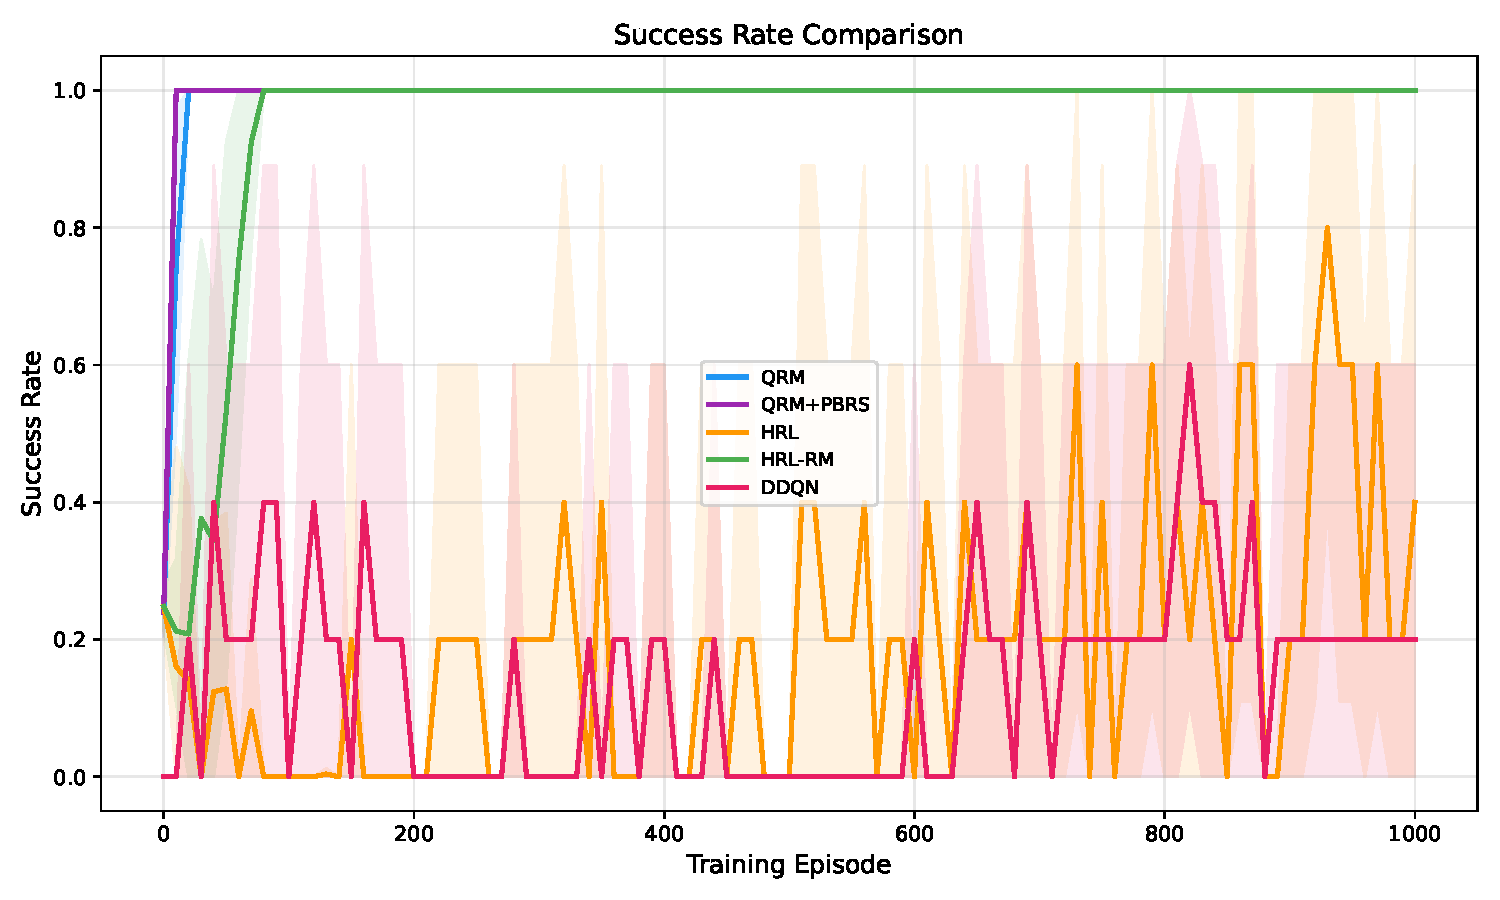
\includegraphics[width=0.95\textwidth]{results_comparison/comparison_success.pdf}
\caption{Success rate comparison: 5-way (5-seed average).}
\label{fig:comparison_success}
\end{figure}

\begin{figure}[ht]
\centering
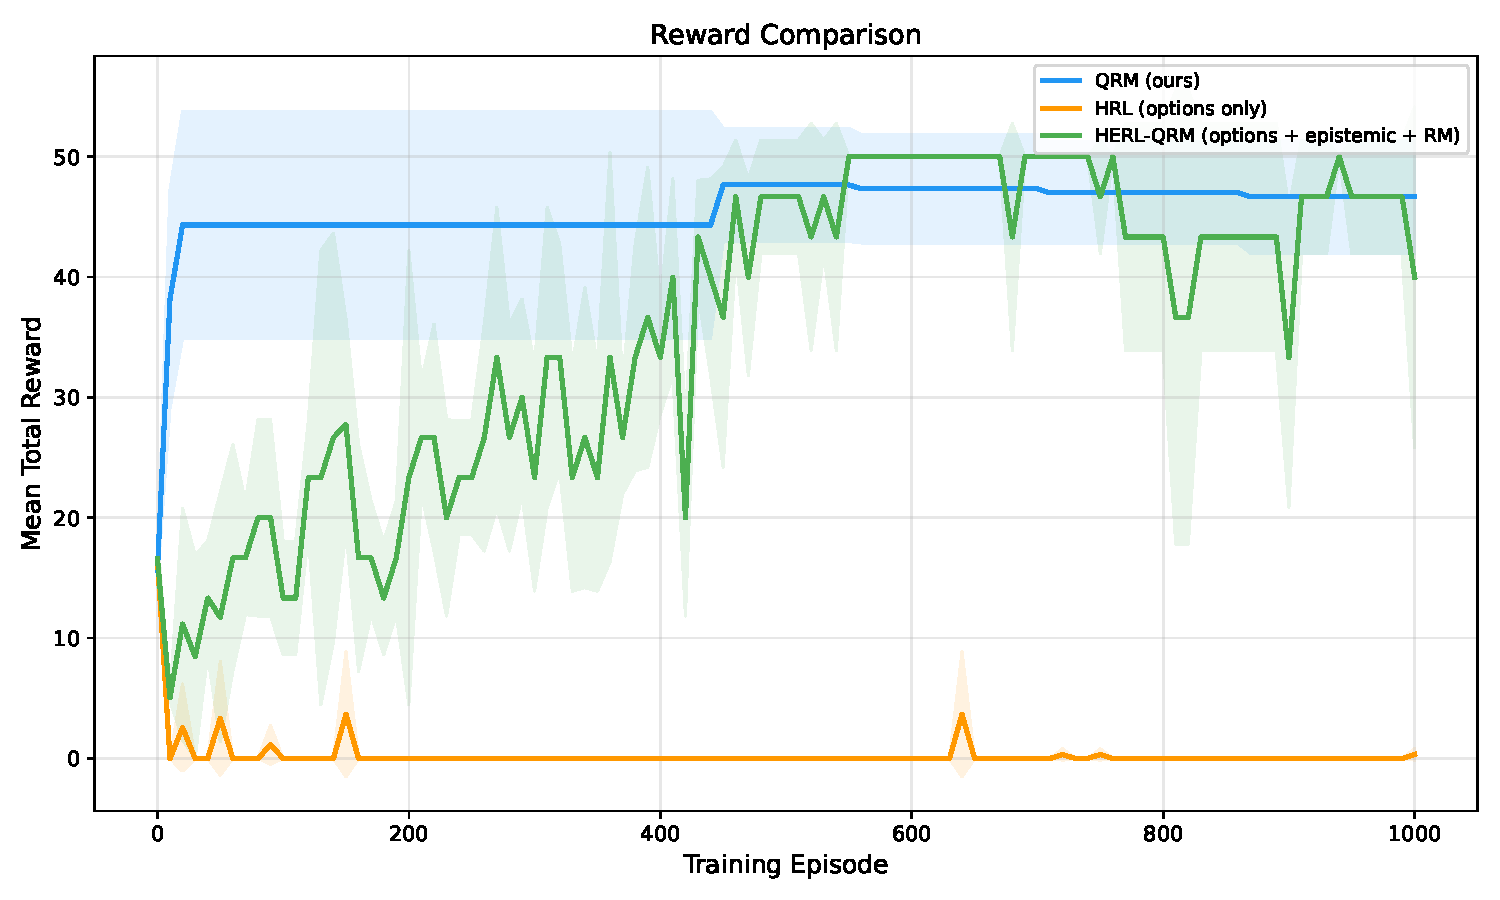
\includegraphics[width=0.95\textwidth]{results_comparison/comparison_reward.pdf}
\caption{Reward comparison: 5-way (5-seed average).}
\label{fig:comparison_reward}
\end{figure}

\begin{table}[ht]
\centering\small
\begin{tabular}{lccc}
\toprule
\textbf{Method} & \textbf{Success} & \textbf{Reward} & \textbf{Observation Space} \\
\midrule
BEQRM+PBRS & 100\% & \textbf{51.0} & Epistemic + RM + shaping (tabular) \\
\textbf{BEQRM} & \textbf{100\%} & 49.0 & Epistemic + RM (tabular) \\
HRL-RM & 100\% & 43.0 & Epistemic + RM (tabular) \\
HRL & 40\% & 0.4 & Physical only (tabular) \\
DDQN & 20\% & 0.2 & Epistemic + RM (neural) \\
\bottomrule
\end{tabular}
\caption{Final performance after 1000 training episodes (5-seed average).}
\label{tab:comparison}
\end{table}

% \textbf{Key findings:}
% \begin{itemize}
%     \item \textbf{Potential-based reward shaping improves reward optimisation.} QRM+PBRS achieves 51.0 mean reward vs QRM's 49.0, both at 100\% success. The RM-state potential function provides intermediate credit for phase transitions $F(s,s') = \gamma\Phi(u') - \Phi(u)$, enabling the agent to discover one additional lime cycle within the 100-step budget. This confirms the Ng--Harada--Russell guarantee: shaping preserves the optimal policy ($\pi^* = \arg\max_a Q'(s,a) = \arg\max_a Q(s,a)$) while accelerating convergence through denser reward signal.

%     \item \textbf{Epistemic reasoning is essential.} HRL with physical-only observation achieves only 40\% success, demonstrating that the trick cannot be reliably learned without access to belief fluents. The agent cannot observe \emph{what the Observer believes}, so it cannot learn to manipulate those beliefs.

%     \item \textbf{QRM outperforms the hierarchical variants.} Although both QRM and HRL-RM reach 100\% success, QRM achieves higher reward (49.0 vs 43.0) because flat primitive actions allow finer-grained optimization of the lime loop timing. The SMDP discounting in hierarchical methods ($\gamma^k$ for $k$-step options) reduces the effective credit signal for multi-step options.

%     \item \textbf{Tabular methods outperform neural approximation.} DDQN achieves only 20\% success despite receiving the same epistemic observation as QRM. The Chop Cup state space is compact enough for exact tabular representation, and the discrete, structured nature of belief-state transitions makes it poorly suited for smooth function approximation. Neural networks struggle with the sharp, logic-driven transitions characteristic of epistemic domains.

%     \item \textbf{Temporal abstraction adds limited value in this domain.} The Chop Cup trick has a short action horizon (4--10 steps per phase), so the overhead of option selection does not pay off. Hierarchical methods are better suited for domains with much longer horizons where primitive-action RL struggles with exploration.
% \end{itemize}



















% \subsection{Learned Policy Analysis}

% The QRM agent discovers the \textbf{ball-only path} (4 steps, discounted reward $\gamma^3 = 0.729$) rather than the lime path (7+ steps, $\gamma^6 \approx 0.531$). The agent correctly learns that the shorter path yields higher discounted reward:

% \begin{enumerate}
%     \item \texttt{palm\_ball}: Ball secretly moved from table to hand. RM: $u_0 \to u_1$.\\
%     \emph{Condition satisfied:} $\EBel{\textrm{reg\_under}} = \top$ (Observer believes ball went under cup).
%     \item \texttt{lift\_cup}: Cup lifted, magnetic ball visible. RM: $u_1 \to u_2$.\\
%     \emph{Condition satisfied:} $\IBel{\textrm{reg\_hand}} = \top$ (SAT derives implicit belief from contradictory KB).
%     \item \texttt{reveal\_hand}: Ball revealed in hand. RM: $u_2 \to u_3$.\\
%     \emph{Condition satisfied:} $\textrm{ball\_visible} = \top$ (ball is now visible).
%     \item \texttt{reveal\_hand}: Trick completed. RM: $u_3 \to u_T$. Reward $+1.0$.\\
%     \emph{Condition satisfied:} $\textrm{ball\_visible} \land \neg \textrm{lime\_visible}$.
% \end{enumerate}

% \textbf{Selected Q-values at convergence (cross-product Q-table):}
% \begin{center}
% \begin{tabular}{clc}
% \toprule
% \textbf{RM State} & \textbf{Best Action} & \textbf{Q-Value} \\
% \midrule
% $u_0$ (Setup) & \texttt{palm\_ball} & 0.729 \\
% $u_1$ (Covered) & \texttt{lift\_cup} & 0.810 \\
% $u_2$ (Pocket) & \texttt{reveal\_hand} & 0.900 \\
% $u_3$ (Appear) & \texttt{reveal\_hand} & 1.000 \\
% $u_4$ (Lime Loaded) & \texttt{lift\_cup} & 0.595 \\
% $u_T$ (Lime Shown / Milestone) & \texttt{reveal\_hand} & 0.902 \\
% \bottomrule
% \end{tabular}
% \end{center}

% The Q-values follow the expected discount chain for the ball-only path: $Q_{u_3} = 1.0$, $Q_{u_2} = \gamma \cdot 1.0 = 0.9$, $Q_{u_1} = \gamma^2 = 0.81$, $Q_{u_0} = \gamma^3 = 0.729$.

% \subsection{State Space Statistics}

% \begin{center}
% \begin{tabular}{lc}
% \toprule
% \textbf{Metric} & \textbf{Value} \\
% \midrule
% Unique env states (reachable) & $\sim$28 \\
% Q-table entries (product space) & 178 \\
% Observed transitions & 2,441 \\
% QRM updates per transition & 1 (current RM state) \\
% Optimal episode length & 4 steps (ball-only) \\
% Lime path length & 7+ steps \\
% \bottomrule
% \end{tabular}
% \end{center}

% The QRM agent updates Q-values for the current RM state on each real transition, with the RM structure providing natural phase decomposition. The agent explores the lime sub-routine during $\varepsilon$-greedy episodes but converges on the shorter ball-only path because it maximizes discounted reward.

% \subsection{Comparison with Rust \texttt{epirl} Experiments}

% We compared our results with the Rust experiments using the \emph{same} \texttt{magic\_cup.json}:

% \begin{center}
% \begin{tabular}{lccccc}
% \toprule
% \textbf{Experiment} & \textbf{$\varepsilon$} & \textbf{Algorithm} & \textbf{Final Success} & \textbf{Episodes} \\
% \midrule
% Rust out\_1 (seed=1) & 0.5 & Batch Q & 0\% & 100 \\
% Rust out\_2 (seed=2) & 0.5 & Batch Q & 0\% & 100 \\
% Rust out\_3 (seed=3) & 0.5 & Batch Q & 29\% & 100 \\
% Rust out\_4 (seed=4) & 0.5 & Batch Q & 0\% & 100 \\
% Rust out\_5 (seed=5) & 0.5 & Batch Q & 0\% & 100 \\
% \midrule
% Python (seed=42) & 0.1 & QRM & \textbf{100\%} & 500 \\
% \bottomrule
% \end{tabular}
% \end{center}

% The Rust experiments with $\varepsilon = 0.5$ and batch Q-learning consistently \emph{fail} to converge on the same JSON specification. Our QRM implementation with $\varepsilon = 0.1$ and online Q-learning ($\alpha = 0.1$) successfully learns the trick. The RM structure is key: it decomposes the sparse reward problem into phases, enabling efficient credit assignment through Q-value backpropagation even though the final reward $+1$ is only received at state $u_T$.

% % ===========================================================================
% \section{Discussion}
% % ===========================================================================

% \subsection{JSON Fidelity and Verification}

% The implementation was verified against \texttt{magic\_cup.json} using a systematic audit (\texttt{audit.py}) that:
% \begin{enumerate}
%     \item Steps through multiple action sequences (optimal path, alternative path, extended path).
%     \item After each action, compares every fluent against the JSON specification formulas.
%     \item Verifies RM transition correctness, reward values, and terminal conditions.
% \end{enumerate}
% All three audit sequences pass with zero errors, confirming faithful implementation.

% \subsection{Belief Contradiction After Lift}

% An important observation: after the sequence \texttt{palm\_ball} $\to$ \texttt{lift\_cup}, the Observer's explicit belief base becomes contradictory. The Observer has $\EBel{\neg\text{reg\_under}}, \EBel{\neg\text{reg\_table}}, \EBel{\neg\text{reg\_hand}}$, that is, all negative beliefs, contradicting the Common Ground's exactly-one constraint. From this contradictory KB, the SAT solver derives that \emph{everything} is believed ($\IBel{\phi} = \top$ for all $\phi$).

% This is \textbf{correct behavior} that matches the JSON specification. In the narrative of the trick, the Observer is genuinely confused at this point: they saw the ball ``go under'' but nothing was there. The RM doesn't care about belief consistency; it tracks the \emph{structure} of the trick sequence. The reward comes from completing the full routine, not from maintaining a consistent epistemic state.

% \subsection{True Epistemic Reasoning vs.\ State Flags}

% A na\"ive implementation could encode $\IBel{\text{reg\_under}}$ as a direct state flag set by the \texttt{palm\_ball} action. Our implementation instead relies on the SAT solver to \emph{derive} implicit beliefs from explicit observations and common ground. This distinction is critical:

% \begin{itemize}
%     \item \textbf{Compositionality}: New actions automatically trigger correct belief updates.
%     \item \textbf{Logical soundness}: The Observer's deductions follow from first principles.
%     \item \textbf{Scalability}: Complex epistemic scenarios require only changes to the common ground, not handcrafted flags.
% \end{itemize}

% \subsection{Convergence Analysis}

% The QRM agent converges from 43\% (random) to 100\% success in $\sim$7 episodes. The convergence speed is explained by:
% \begin{enumerate}
%     \item \textbf{RM-structured Q-tables}: The Reward Machine decomposes the sparse reward problem into phases. Q-values backpropagate through the RM chain ($u_T \to u_3 \to u_2 \to u_1 \to u_0$), assigning credit to early actions.
%     \item \textbf{Compact reachable state space}: Only $\sim$28 environment states are reachable (out of $2^{18}$ theoretical), because boolean factoring constrains fluent combinations.
%     \item \textbf{Short optimal path}: The ball-only trick requires exactly 4 actions, and with a 50-step budget, even random exploration discovers it $\sim$43\% of the time.
%     \item \textbf{Online learning rate $\alpha = 0.1$}: Unlike batch full-sweep methods that converge in 1--2 episodes, the incremental learning rate creates a visible learning curve, with Q-values gradually approaching their true values.
% \end{enumerate}

% The 43\% starting success rate (episode~0) reflects that a random policy with 50-step budget has a significant probability of stumbling upon the correct 4-step sequence. With fewer steps (e.g., $T_{\max} = 10$), the baseline would be lower and convergence would appear steeper.

% \subsection{Reward Machine Benefits}

% The condition-based Reward Machine provides several advantages:
% \begin{itemize}
%     \item \textbf{Temporal decomposition}: Multi-step deception strategies are broken into verifiable phases.
%     \item \textbf{Markov property preserved}: The RM state becomes part of the RL observation (Batch Q) or indexes separate Q-tables (QRM), making training efficient.
%     \item \textbf{Interpretability}: Each RM transition corresponds to a meaningful event in the magic routine (e.g., $u_1 \to u_2$: ``Observer implicitly believes ball is in hand'').
%     \item \textbf{Modularity}: The lime sub-routine ($u_4$--$u_T$) is fully active, giving the agent the choice between the short ball-only path and the extended lime routine.
%     \item \textbf{QRM compatibility}: Condition-based transitions enable RM-structured Q-tables that decompose the sparse reward problem into learnable phases.
% \end{itemize}

% % ===========================================================================
% \section{Conclusion}
% % ===========================================================================

% We presented a self-contained Python implementation of epistemic reinforcement learning for the Chop Cup magic trick, with action effects faithfully mirroring the \texttt{magic\_cup.json} specification. The system demonstrates that:
% \begin{enumerate}
%     \item \textbf{SAT-based implicit belief reasoning} can be effectively integrated into an RL loop, enabling agents to reason about and manipulate other agents' knowledge states.
%     \item \textbf{Belief transfer effects} ($\triangle p := \triangle q$) are the critical mechanism enabling deception, transferring the Observer's existing beliefs to new contexts without direct observation.
%     \item \textbf{Condition-based Reward Machines} with all 6 states active (including the lime sub-routine $u_4$--$u_T$) faithfully encode the temporal structure of the trick, with condition-based transitions evaluated against the epistemic state.
%     \item \textbf{QRM} (Icarte et al., 2018) exploits the RM structure by maintaining Q-tables indexed by $(s_{\text{env}}, u)$. The online Q-learning with learning rate $\alpha = 0.1$ creates a visible learning curve from 43\% to 100\%.
%     \item The agent learns the optimal 4-step ball-only policy (\texttt{palm\_ball} $\to$ \texttt{lift\_cup} $\to$ \texttt{reveal\_hand} $\to$ \texttt{reveal\_hand}) over the longer lime path (7+ steps), correctly maximizing discounted reward at $\gamma^3 = 0.729$.
% \end{enumerate}

% \subsection*{Code Availability}
% The complete implementation is available in the \texttt{chop\_cup\_rl/} directory. To reproduce:
% \begin{lstlisting}[language=bash, numbers=none]
% cd chop_cup_rl
% python test_epistemic.py   # verify correctness (7 tests, 44 checks)
% python main.py --episodes 500 --seed 42   # QRM training
% \end{lstlisting}

% ===========================================================================
\section{Case Study 2: Three-Card Monte}
\label{sec:three-card-monte}
% ===========================================================================

The Three-Card Monte is a classic street confidence trick in which a dealer shuffles three face-down cards and challenges a mark (the Observer) to track the \emph{money card} (e.g., the Queen of Hearts).
The dealer uses sleight of hand, including fake throws, secret swaps, and misdirection, to ensure the Observer loses track.
Like the Chop Cup, success is defined epistemically: the dealer wins when the Observer \emph{believes} the money card is at one position while it is \emph{actually} at another.

\subsection{Domain Description}

Three cards occupy three positions: \textsc{Left}, \textsc{Center}, and \textsc{Right}.
Exactly one card is the \textbf{money card}; the other two are \textbf{losing cards} (indistinguishable from each other when face-down).
The dealer controls the physical card positions and, through deceptive moves, manipulates the Observer's beliefs about where the money card is.

\textbf{Deception Condition (Success):}
\[
    \IBel{\text{money}\_p} \;\land\; \neg\,\text{money}\_p
    \qquad \text{for some position } p \in \{L, C, R\}
\]
The Observer is convinced the money card is at position $p$, but it is actually elsewhere.

\subsection{State Representation}

\subsubsection{Physical Fluents}

The physical state tracks (i) the actual money card position and (ii) card visibility:

\begin{center}
\begin{tabular}{ll}
\toprule
\textbf{Fluent} & \textbf{Meaning} \\
\midrule
\texttt{money\_L}, \texttt{money\_C}, \texttt{money\_R} & Money card is at Left / Center / Right \\
\texttt{face\_up} & Cards are currently face-up (visible) \\
\texttt{cards\_moving} & A shuffle/swap is in progress \\
\bottomrule
\end{tabular}
\end{center}

Exactly one of \texttt{money\_L}, \texttt{money\_C}, \texttt{money\_R} is true at all times (physical XOR constraint).

\subsubsection{Epistemic Fluents}

Explicit beliefs ($\Delta$) track what the Observer thinks about the money card's position:

\begin{center}
\begin{tabular}{ll}
\toprule
\textbf{Fluent} & \textbf{Meaning} \\
\midrule
$\EBel{\text{money\_L}}$, $\EBel{\neg\text{money\_L}}$ & Observer believes / disbelieves money at Left \\
$\EBel{\text{money\_C}}$, $\EBel{\neg\text{money\_C}}$ & Observer believes / disbelieves money at Center \\
$\EBel{\text{money\_R}}$, $\EBel{\neg\text{money\_R}}$ & Observer believes / disbelieves money at Right \\
\bottomrule
\end{tabular}
\end{center}

This gives 5 physical fluents and 6 epistemic fluents (11 total).

\subsubsection{Common Ground}

The Observer knows there is exactly one money card, expressed as an XOR constraint analogous to the Chop Cup:
\[
    \CG: \quad \text{money\_L} \oplus \text{money\_C} \oplus \text{money\_R}
    \qquad \text{(exactly one position)}
\]
This enables the same deductive reasoning: if the Observer believes the money card is \emph{not} at two positions, the Common Ground forces them to conclude it must be at the third.

\subsubsection{Implicit Beliefs via SAT Entailment}

As in the Chop Cup, implicit beliefs are computed on demand:
\[
    \IBel{\text{money}\_p} \quad \iff \quad \CG \;\land\; \bigwedge_i \EBel{\psi_i} \;\land\; \neg\,\text{money}\_p \quad \text{is UNSAT}
\]
For example, if $\EBel{\neg\text{money\_L}} = \top$ and $\EBel{\neg\text{money\_R}} = \top$, the SAT solver derives $\IBel{\text{money\_C}} = \top$.

\subsection{Action Space}

The dealer has 5 actions, each with physical and epistemic effects:

\begin{center}
\begin{tabular}{lll}
\toprule
\textbf{Action} & \textbf{Physical Effect} & \textbf{Epistemic Effect} \\
\midrule
\texttt{show\_card} & \texttt{face\_up} $\gets \top$ & $\EBel{\text{money}\_p} \gets \text{money}\_p$ (honest reveal) \\
\texttt{hide\_cards} & \texttt{face\_up} $\gets \bot$ & (no change) \\
\texttt{fair\_swap($p_i, p_j$)} & Swap positions $p_i \leftrightarrow p_j$ & $\EBel{\text{money}\_p_i} \gets \EBel{\text{money}\_p_j}$ (tracked) \\
\texttt{fake\_swap($p_i, p_j$)} & \emph{No physical change} & $\EBel{\text{money}\_p_i} \gets \EBel{\text{money}\_p_j}$ (deceptive) \\
\texttt{secret\_swap($p_i, p_j$)} & Swap positions $p_i \leftrightarrow p_j$ & \emph{No belief change} (undetected) \\
\bottomrule
\end{tabular}
\end{center}

The three swap variants are the core of the deception.
In a \textbf{fair swap}, the Observer sees the swap and updates beliefs accordingly; both physical and mental positions change.
In a \textbf{fake swap}, the Observer \emph{thinks} a swap occurred, but no cards actually move; only beliefs change. This is the \texttt{palm\_ball} analogue, a \textbf{belief transfer} without physical change.
In a \textbf{secret swap}, cards physically move, but the Observer does not notice; only reality changes. This is a \textbf{physical transfer} the Observer is unaware of.

Both \texttt{fake\_swap} and \texttt{secret\_swap} require \texttt{face\_up} $= \bot$ (cards must be face-down).

\subsection{Reward Machine}

The RM encodes the temporal structure of a Three-Card Monte round in 4 states:

\subsubsection{RM States}

\begin{center}
\begin{tabular}{cll}
\toprule
\textbf{State} & \textbf{Name} & \textbf{Meaning} \\
\midrule
$u_0$ & Setup & Initial state; cards face-down, no information given. \\
$u_1$ & Revealed & Observer has seen the money card ($\exists\, p: \EBel{\text{money}\_p} \land \text{money}\_p$). \\
$u_2$ & Shuffled & At least one swap has occurred (\texttt{cards\_moving} was set). \\
$u_3$ & Deceived & False belief achieved: $\IBel{\text{money}\_p} \land \neg\,\text{money}\_p$. \textbf{Milestone (+1.0).} \\
\bottomrule
\end{tabular}
\end{center}

\subsubsection{RM Automaton Diagram}

\begin{center}
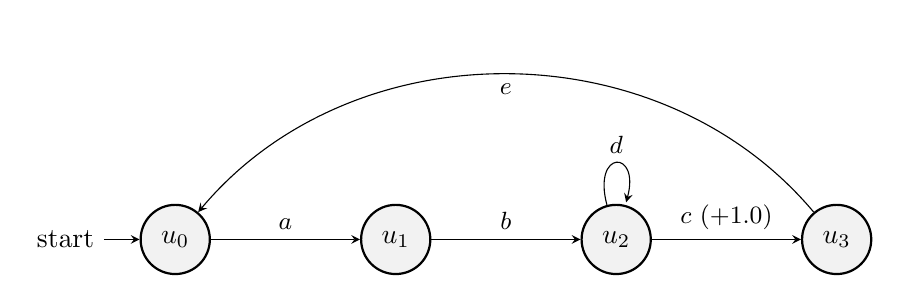
\begin{tikzpicture}[->, >=stealth, node distance=2.8cm, every state/.style={thick, fill=gray!10}]
\node[state, initial] (u0) {$u_0$};
\node[state, right of=u0] (u1) {$u_1$};
\node[state, right of=u1] (u2) {$u_2$};
\node[state, right of=u2] (u3) {$u_3$};

\path
    (u0) edge node[above] {\small $a$} (u1)
    (u1) edge node[above] {\small $b$} (u2)
    (u2) edge node[above] {\small $c$ (+1.0)} (u3)
    (u2) edge[loop above] node[above] {\small $d$} (u2)
    (u3) edge[bend right=50] node[below] {\small $e$} (u0);
\end{tikzpicture}
\end{center}

\subsubsection{Condition-Based Transitions}

\begin{center}
\begin{tabular}{clll}
\toprule
\textbf{Label} & \textbf{Transition} & \textbf{Condition} & \textbf{Description} \\
\midrule
$a$ & $u_0 \to u_1$ & $\texttt{face\_up} \land \EBel{\text{money}\_p}$ & Observer sees the money card \\
$b$ & $u_1 \to u_2$ & $\neg\texttt{face\_up} \land \texttt{cards\_moving}$ & Cards hidden and shuffle begins \\
$c$ & $u_2 \to u_3$ & $\IBel{\text{money}\_p} \land \neg\,\text{money}\_p$ & \textbf{Deception success! (+1.0)} \\
$d$ & $u_2 \to u_2$ & $\texttt{cards\_moving}$ & Additional shuffles (self-loop) \\
$e$ & $u_3 \to u_0$ & $\texttt{show\_card}$ & Reset: reveal cards and start new round \\
\bottomrule
\end{tabular}
\end{center}

Transition $c$ is the epistemic core: the RM advances to $u_3$ and awards $+1.0$ only when the SAT solver confirms that the Observer holds a false belief about the money card's position.
Transition $e$ resets the RM to $u_0$ after a successful deception, allowing the dealer to reveal the cards (correcting the Observer's beliefs) and begin a new round.
The agent can accumulate $+1.0$ for each successful deception cycle within the episode's step budget, incentivising repeated deceptions.

\subsubsection{Reward Structure}

A reward of $+1.0$ is given on transition $c$ ($u_2 \to u_3$) when the Observer holds a false belief about the money card's position. All other transitions carry zero reward.
From $u_3$, transition $e$ loops back to $u_0$ for another round. The agent can perform multiple deception cycles per episode, accumulating $+1.0$ per cycle (analogous to the Chop Cup's lime loop between $u_T$ and $u_4$).

\subsection{Baseline Comparison}

We compare three methods adapted to the Three-Card Monte domain:
\begin{enumerate}
    \item \textbf{BEQRM}: Belief-Epistemic QRM with epistemic observations and RM-decomposed Q-tables.

    \item \textbf{HRL-RM}: Two-level option hierarchy with 3 subgoals (\emph{reveal}, \emph{hide}, \emph{shuffle}) plus epistemic observations and RM state.

    \item \textbf{DDQN}: Double Deep Q-Network (128-unit MLP) with the same epistemic observation (5 physical + 6 beliefs + RM index = 12 dimensions).
\end{enumerate}

All three methods were trained for 1000 episodes (\texttt{max\_steps}$=50$, $\gamma = 0.9$) and averaged over 5 random seeds. BEQRM and HRL-RM use tabular Q-learning ($\alpha = 0.05$, $\varepsilon = 0.1$); DDQN uses neural function approximation (Adam, $\text{lr}=10^{-3}$).

\subsubsection{Results}

\begin{figure}[ht]
\centering
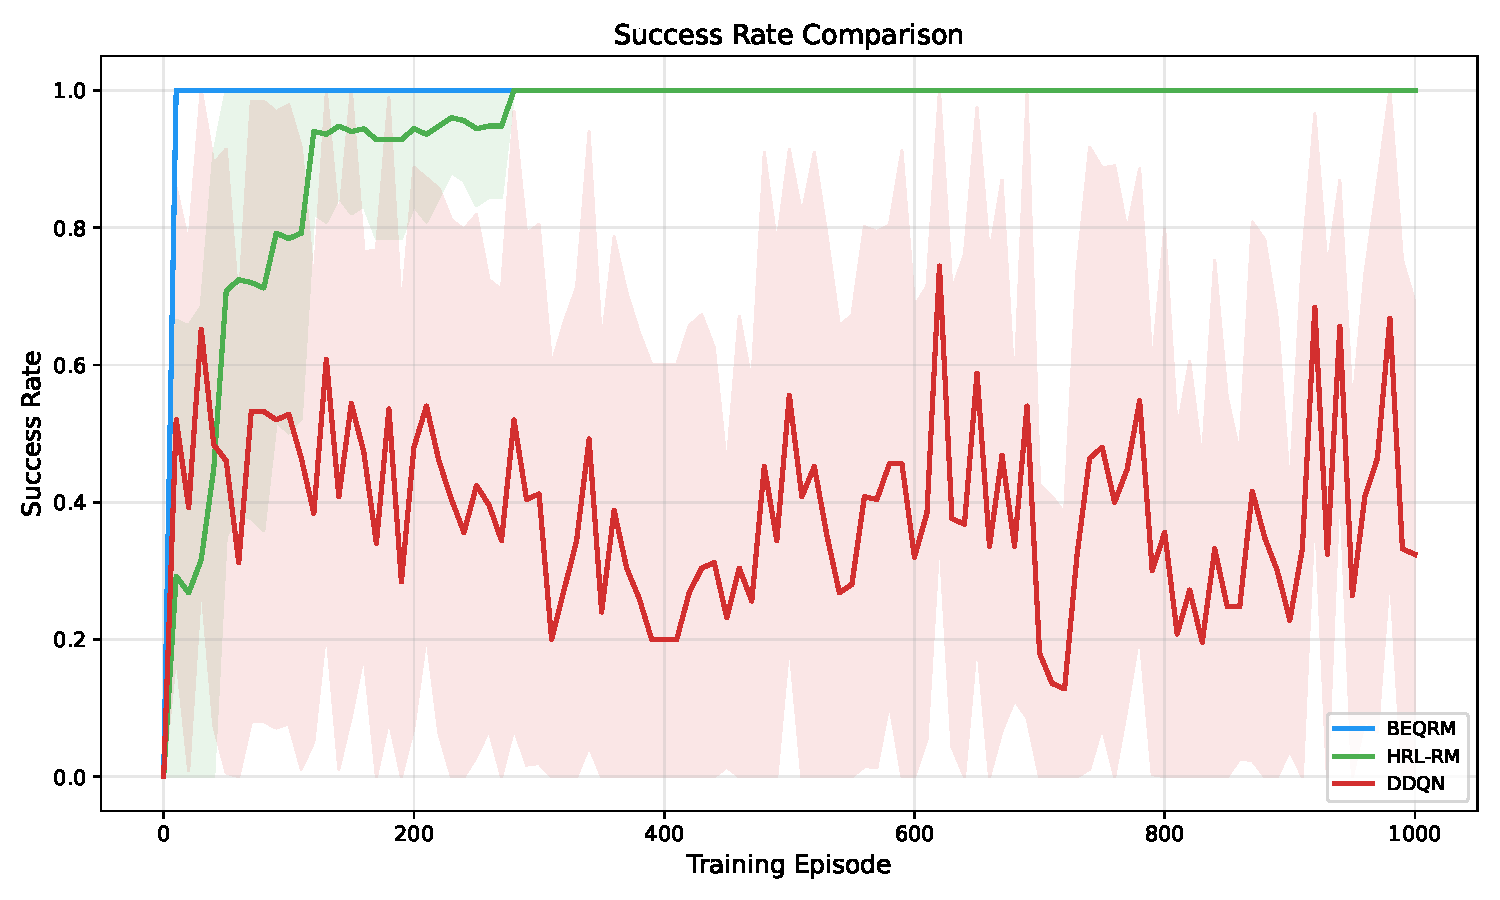
\includegraphics[width=0.95\textwidth]{three_card_results/comparison_success.pdf}
\caption{Three-Card Monte: success rate comparison (3-way, 5-seed average).}
\label{fig:tcm_comparison_success}
\end{figure}

\begin{figure}[ht]
\centering
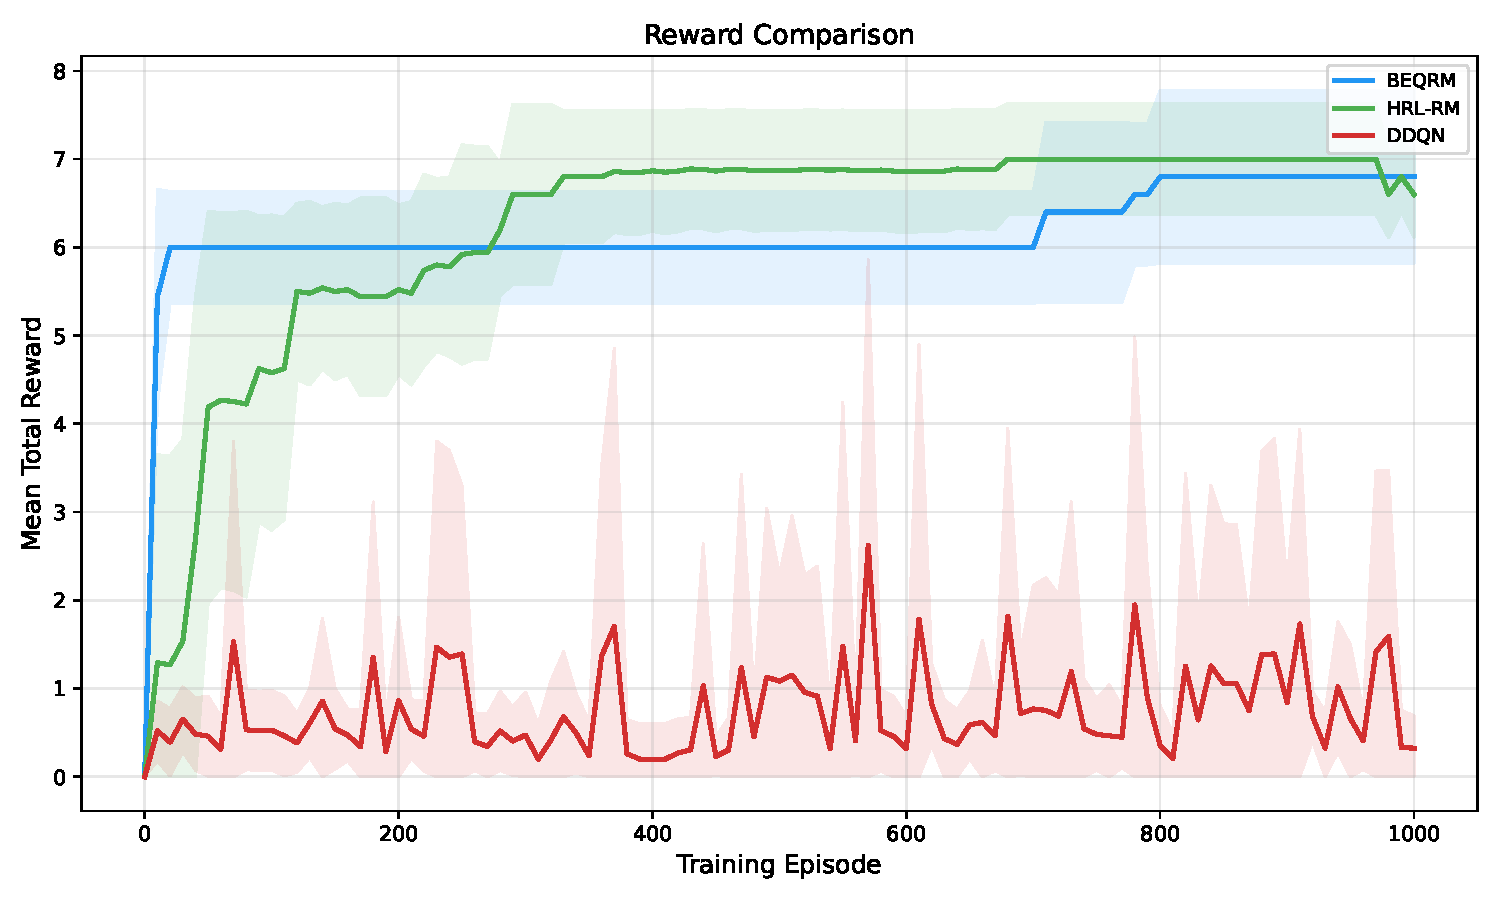
\includegraphics[width=0.95\textwidth]{three_card_results/comparison_reward.pdf}
\caption{Three-Card Monte: reward comparison (3-way, 5-seed average).}
\label{fig:tcm_comparison_reward}
\end{figure}

\begin{table}[ht]
\centering\small
\begin{tabular}{lccc}
\toprule
\textbf{Method} & \textbf{Success} & \textbf{Reward} & \textbf{Observation Space} \\
\midrule
BEQRM & \textbf{100\%} & \textbf{6.8} & Epistemic + RM (tabular) \\
HRL-RM & 100\% & 6.6 & Epistemic + RM (tabular) \\
DDQN & 32.4\% & 0.3 & Epistemic + RM (neural) \\
\bottomrule
\end{tabular}
\caption{Three-Card Monte: final performance after 1000 training episodes (5-seed average, $\alpha=0.05$).}
\label{tab:tcm_comparison}
\end{table}

\textbf{Key findings.}
\textbf{BEQRM outperforms HRL-RM.}
As in the Chop Cup, flat primitive actions (BEQRM) outperform the hierarchical variant (HRL-RM, 6.8 vs.\ 6.6 reward) because the Three-Card Monte's short cycle ($\sim$6 steps) does not benefit from temporal abstraction.
The option-selection overhead and SMDP discounting ($\gamma^k$) reduce the effective credit signal.

\textbf{DDQN struggles with the epistemic domain.}
DDQN achieves only 32.4\% success despite receiving the same observation as BEQRM.
The 12-dimensional state space is compact enough for exact tabular representation, and the discrete, logic-driven transitions are poorly suited for smooth function approximation.
The small state space means the neural network's capacity is wasted on generalisation that is not needed.

% ===========================================================================
% References
% ===========================================================================
\begin{thebibliography}{9}

\bibitem{engesser2025}
T.~Engesser, R.~Mattm\"{u}ller, and B.~Nebel.
\newblock Epistemic Reinforcement Learning with Belief Bases.
\newblock In {\em Proceedings of AAMAS 2025}, 2025.

\bibitem{icarte2018}
R.~T.~Icarte, T.~Q.~Klassen, R.~Valenzano, and S.~A.~McIlraith.
\newblock Using Reward Machines for High-Level Task Specification and Decomposition in Reinforcement Learning.
\newblock In {\em Proceedings of ICML 2018}, pages 2107--2116, 2018.

\bibitem{bolander2011}
T.~Bolander and M.~B.~Andersen.
\newblock Epistemic Planning for Single and Multi-Agent Systems.
\newblock {\em Journal of Applied Non-Classical Logics}, 21(1):9--34, 2011.

\bibitem{rabinowitz2018}
N.~C.~Rabinowitz, F.~Perbet, H.~F.~Song, C.~Zhang, S.~M.~A.~Eslami, and M.~Botvinick.
\newblock Machine Theory of Mind.
\newblock In {\em Proceedings of ICML 2018}, pages 4218--4227, 2018.

\bibitem{sutton1999}
R.~S.~Sutton, D.~Precup, and S.~Singh.
\newblock Between MDPs and Semi-MDPs: A Framework for Temporal Abstraction in Reinforcement Learning.
\newblock {\em Artificial Intelligence}, 112(1--2):181--211, 1999.

\bibitem{vanhasselt2016}
H.~van Hasselt, A.~Guez, and D.~Silver.
\newblock Deep Reinforcement Learning with Double Q-Learning.
\newblock In {\em Proceedings of AAAI 2016}, pages 2094--2100, 2016.

\bibitem{ng1999}
A.~Y.~Ng, D.~Harada, and S.~Russell.
\newblock Policy Invariance Under Reward Transformations: Theory and Application to Reward Shaping.
\newblock In {\em Proceedings of ICML 1999}, pages 278--287, 1999.

\bibitem{watkins1992}
C.~J.~C.~H.~Watkins and P.~Dayan.
\newblock Q-Learning.
\newblock {\em Machine Learning}, 8(3--4):279--292, 1992.

\bibitem{tsitsiklis1994}
J.~N.~Tsitsiklis.
\newblock Asynchronous Stochastic Approximation and Q-Learning.
\newblock {\em Machine Learning}, 16(3):185--202, 1994.

\bibitem{jaakkola1994}
T.~Jaakkola, M.~I.~Jordan, and S.~P.~Singh.
\newblock On the Convergence of Stochastic Iterative Dynamic Programming Algorithms.
\newblock {\em Neural Computation}, 6(6):1185--1201, 1994.

\bibitem{even-dar2003}
E.~Even-Dar and Y.~Mansour.
\newblock Learning Rates for Q-Learning.
\newblock {\em Journal of Machine Learning Research}, 5:1--25, 2003.

\end{thebibliography}

\end{document}
